% Options for packages loaded elsewhere
\PassOptionsToPackage{unicode}{hyperref}
\PassOptionsToPackage{hyphens}{url}
\documentclass[
]{article}
\usepackage{xcolor}
\usepackage[margin=1in]{geometry}
\usepackage{amsmath,amssymb}
\setcounter{secnumdepth}{5}
\usepackage{iftex}
\ifPDFTeX
  \usepackage[T1]{fontenc}
  \usepackage[utf8]{inputenc}
  \usepackage{textcomp} % provide euro and other symbols
\else % if luatex or xetex
  \usepackage{unicode-math} % this also loads fontspec
  \defaultfontfeatures{Scale=MatchLowercase}
  \defaultfontfeatures[\rmfamily]{Ligatures=TeX,Scale=1}
\fi
\usepackage{lmodern}
\ifPDFTeX\else
  % xetex/luatex font selection
\fi
% Use upquote if available, for straight quotes in verbatim environments
\IfFileExists{upquote.sty}{\usepackage{upquote}}{}
\IfFileExists{microtype.sty}{% use microtype if available
  \usepackage[]{microtype}
  \UseMicrotypeSet[protrusion]{basicmath} % disable protrusion for tt fonts
}{}
\makeatletter
\@ifundefined{KOMAClassName}{% if non-KOMA class
  \IfFileExists{parskip.sty}{%
    \usepackage{parskip}
  }{% else
    \setlength{\parindent}{0pt}
    \setlength{\parskip}{6pt plus 2pt minus 1pt}}
}{% if KOMA class
  \KOMAoptions{parskip=half}}
\makeatother
\usepackage{color}
\usepackage{fancyvrb}
\newcommand{\VerbBar}{|}
\newcommand{\VERB}{\Verb[commandchars=\\\{\}]}
\DefineVerbatimEnvironment{Highlighting}{Verbatim}{commandchars=\\\{\}}
% Add ',fontsize=\small' for more characters per line
\usepackage{framed}
\definecolor{shadecolor}{RGB}{248,248,248}
\newenvironment{Shaded}{\begin{snugshade}}{\end{snugshade}}
\newcommand{\AlertTok}[1]{\textcolor[rgb]{0.94,0.16,0.16}{#1}}
\newcommand{\AnnotationTok}[1]{\textcolor[rgb]{0.56,0.35,0.01}{\textbf{\textit{#1}}}}
\newcommand{\AttributeTok}[1]{\textcolor[rgb]{0.13,0.29,0.53}{#1}}
\newcommand{\BaseNTok}[1]{\textcolor[rgb]{0.00,0.00,0.81}{#1}}
\newcommand{\BuiltInTok}[1]{#1}
\newcommand{\CharTok}[1]{\textcolor[rgb]{0.31,0.60,0.02}{#1}}
\newcommand{\CommentTok}[1]{\textcolor[rgb]{0.56,0.35,0.01}{\textit{#1}}}
\newcommand{\CommentVarTok}[1]{\textcolor[rgb]{0.56,0.35,0.01}{\textbf{\textit{#1}}}}
\newcommand{\ConstantTok}[1]{\textcolor[rgb]{0.56,0.35,0.01}{#1}}
\newcommand{\ControlFlowTok}[1]{\textcolor[rgb]{0.13,0.29,0.53}{\textbf{#1}}}
\newcommand{\DataTypeTok}[1]{\textcolor[rgb]{0.13,0.29,0.53}{#1}}
\newcommand{\DecValTok}[1]{\textcolor[rgb]{0.00,0.00,0.81}{#1}}
\newcommand{\DocumentationTok}[1]{\textcolor[rgb]{0.56,0.35,0.01}{\textbf{\textit{#1}}}}
\newcommand{\ErrorTok}[1]{\textcolor[rgb]{0.64,0.00,0.00}{\textbf{#1}}}
\newcommand{\ExtensionTok}[1]{#1}
\newcommand{\FloatTok}[1]{\textcolor[rgb]{0.00,0.00,0.81}{#1}}
\newcommand{\FunctionTok}[1]{\textcolor[rgb]{0.13,0.29,0.53}{\textbf{#1}}}
\newcommand{\ImportTok}[1]{#1}
\newcommand{\InformationTok}[1]{\textcolor[rgb]{0.56,0.35,0.01}{\textbf{\textit{#1}}}}
\newcommand{\KeywordTok}[1]{\textcolor[rgb]{0.13,0.29,0.53}{\textbf{#1}}}
\newcommand{\NormalTok}[1]{#1}
\newcommand{\OperatorTok}[1]{\textcolor[rgb]{0.81,0.36,0.00}{\textbf{#1}}}
\newcommand{\OtherTok}[1]{\textcolor[rgb]{0.56,0.35,0.01}{#1}}
\newcommand{\PreprocessorTok}[1]{\textcolor[rgb]{0.56,0.35,0.01}{\textit{#1}}}
\newcommand{\RegionMarkerTok}[1]{#1}
\newcommand{\SpecialCharTok}[1]{\textcolor[rgb]{0.81,0.36,0.00}{\textbf{#1}}}
\newcommand{\SpecialStringTok}[1]{\textcolor[rgb]{0.31,0.60,0.02}{#1}}
\newcommand{\StringTok}[1]{\textcolor[rgb]{0.31,0.60,0.02}{#1}}
\newcommand{\VariableTok}[1]{\textcolor[rgb]{0.00,0.00,0.00}{#1}}
\newcommand{\VerbatimStringTok}[1]{\textcolor[rgb]{0.31,0.60,0.02}{#1}}
\newcommand{\WarningTok}[1]{\textcolor[rgb]{0.56,0.35,0.01}{\textbf{\textit{#1}}}}
\usepackage{graphicx}
\makeatletter
\newsavebox\pandoc@box
\newcommand*\pandocbounded[1]{% scales image to fit in text height/width
  \sbox\pandoc@box{#1}%
  \Gscale@div\@tempa{\textheight}{\dimexpr\ht\pandoc@box+\dp\pandoc@box\relax}%
  \Gscale@div\@tempb{\linewidth}{\wd\pandoc@box}%
  \ifdim\@tempb\p@<\@tempa\p@\let\@tempa\@tempb\fi% select the smaller of both
  \ifdim\@tempa\p@<\p@\scalebox{\@tempa}{\usebox\pandoc@box}%
  \else\usebox{\pandoc@box}%
  \fi%
}
% Set default figure placement to htbp
\def\fps@figure{htbp}
\makeatother
% definitions for citeproc citations
\NewDocumentCommand\citeproctext{}{}
\NewDocumentCommand\citeproc{mm}{%
  \begingroup\def\citeproctext{#2}\cite{#1}\endgroup}
\makeatletter
 % allow citations to break across lines
 \let\@cite@ofmt\@firstofone
 % avoid brackets around text for \cite:
 \def\@biblabel#1{}
 \def\@cite#1#2{{#1\if@tempswa , #2\fi}}
\makeatother
\newlength{\cslhangindent}
\setlength{\cslhangindent}{1.5em}
\newlength{\csllabelwidth}
\setlength{\csllabelwidth}{3em}
\newenvironment{CSLReferences}[2] % #1 hanging-indent, #2 entry-spacing
 {\begin{list}{}{%
  \setlength{\itemindent}{0pt}
  \setlength{\leftmargin}{0pt}
  \setlength{\parsep}{0pt}
  % turn on hanging indent if param 1 is 1
  \ifodd #1
   \setlength{\leftmargin}{\cslhangindent}
   \setlength{\itemindent}{-1\cslhangindent}
  \fi
  % set entry spacing
  \setlength{\itemsep}{#2\baselineskip}}}
 {\end{list}}
\usepackage{calc}
\newcommand{\CSLBlock}[1]{\hfill\break\parbox[t]{\linewidth}{\strut\ignorespaces#1\strut}}
\newcommand{\CSLLeftMargin}[1]{\parbox[t]{\csllabelwidth}{\strut#1\strut}}
\newcommand{\CSLRightInline}[1]{\parbox[t]{\linewidth - \csllabelwidth}{\strut#1\strut}}
\newcommand{\CSLIndent}[1]{\hspace{\cslhangindent}#1}
\setlength{\emergencystretch}{3em} % prevent overfull lines
\providecommand{\tightlist}{%
  \setlength{\itemsep}{0pt}\setlength{\parskip}{0pt}}
\usepackage{array}
\usepackage{longtable}
\usepackage{booktabs}
\usepackage{multirow}
\usepackage{wrapfig}
\usepackage{float}
\usepackage{colortbl}
\usepackage{pdflscape}
\usepackage{tabu}
\usepackage{threeparttable}
\usepackage{threeparttablex}
\usepackage[normalem]{ulem}
\usepackage{makecell}
\usepackage{xcolor}
\usepackage{bookmark}
\IfFileExists{xurl.sty}{\usepackage{xurl}}{} % add URL line breaks if available
\urlstyle{same}
\hypersetup{
  pdftitle={Supporting Information},
  hidelinks,
  pdfcreator={LaTeX via pandoc}}

\title{Supporting Information}
\author{}
\date{\vspace{-2.5em}}

\begin{document}
\maketitle

{
\setcounter{tocdepth}{2}
\tableofcontents
}
\newpage

\section{Supporting Information Text}\label{supporting-information-text}

\subsection{Multi-species functional response (MSFR)
model}\label{multi-species-functional-response-msfr-model}

\subsubsection{MSFR model prior
distributions}\label{msfr-model-prior-distributions}

Below are the vague prior distributions used for MSFR model parameters.
To help with model convergence, we estimate the attack rate, \(b_i\), on
the log scale. Since a uniform prior on the log-transformed scale is no
longer uniform on the real scale, we conduct a prior sensitivity
analysis for the \(\text{log}(b_i)\) prior (section 1.1.6).

Handling time of species \(i\):

\[
h_i \sim \text{Uniform}(0, 1000)
\]

Log-scale attack rate for species \(i\):

\[
\text{log}(b_i) \sim \text{Uniform}(-100, 100)
\]

MSFR exponent:

\[
q \sim \text{Uniform}(-2, 2)
\]

Abundance of available Pacific lamprey at time \(t\):

\[
L_t^A \sim \text{Uniform}(0, 1000000)
\]

Abundance of available Chinook salmon at time \(t\):

\[
S_t^A \sim \text{Uniform}(0, 1000000)
\]

Beta distribution shape parameters informing the lamprey probability of
detection in visual fish ladder surveys:

\[
\alpha^D \sim \text{Uniform}(0, 100)
\] \[
\beta^D \sim \text{Uniform}(0, 100)
\]

\newpage

\subsubsection{MSFR data sources}\label{msfr-data-sources}

Here we outline the data sources used to fit the multi-species
functional response model (MSFR, Equations 8-18). The model uses two
sources of data: 1) gastro-intestinal consumption data from 107
euthanized California sea lions (CSL) and 2) Bonneville dam passage data
from day-time visual counts in fish ladders, night-time visual counts in
fish ladders, and mechanical counts in lamprey passage structures (LPS).
The dam passage data is used to inform both 1) the observed abundance of
fish passed, \(L^P_t\) and \(S^P_t\), during the time window, \(t\) sea
lion euthanasia occurred and 2) the probability of lamprey detection in
day-time visual counts in fish ladders.

To estimate CSL consumption rates, we use data on prey items recovered
in the gastro-intestinal tracks of 107 California sea lions euthanized
below Bonneville dam in 2017-2019 and 2021-2023 (Table S3, Table S6).
This diet analysis is based on the identification of undigested prey
remains from the stomachs and large intestines of euthanized CSLs
following the procedures in Lance et al.~(2001), where prey were
enumerated by examining all structures (otoliths, tail structures,
cephalopod beaks, etc.) to determine the minimum number of individual
prey items in the sample (Lance et al. 2001). These data were retrieved
from annual reports to the National Marine Fisheries Service (NMFS)
documenting compliance with the terms and conditions of the
authorization for lethal removal of California sea lions under the
Marine Mammal Protection Act (Clark et al. 2021, 2023; Edwards et al.
2022).

While above-surface pinniped predation events are monitored at
Bonneville dam and have previously been used to estimate the CSL
functional response for salmonid prey (Hatch, Lessard, and Whiteaker
2018), these above-surface data likely underestimate lamprey predation,
as lamprey predation typically occurs below surface (Tidwell, Braun, and
Leeuw 2023). We therefore use the gastro-intestinal data to reduce
differences in consumption observation error between fish species. We
subset the prey item data to those identified as adult Chinook salmon
and Pacific lamprey, and we assume the prey items represent consumption
in the 24 hours before euthanasia, as this is the time typically taken
for CSL prey to pass through the digestive system (Tidwell, personal
communication).

To estimate the abundance of the prey available to CSL during the period
of consumption, \(L_t^A\) and \(S_t^A\), we use fish passage data from
Bonneville dam. For Chinook salmon, these data include daily, visual
daytime counts across all Bonneville dam fish ladders, retrieved from
the Columbia River DART database
(\url{https://www.cbr.washington.edu/dart/query/adult_graph_text}). For
Pacific lamprey, however, these visual daytime counts in the fish
ladders underestimate abundance, as 1) Pacific lamprey also use Lamprey
Passage Structures (LPS) in addition to the fish ladders and 2) lamprey
tend to migrate at night, rather than during the day (Cates, McClain,
and Gibbons 2020) (Figure 2). These lamprey passage structures (LPS) use
a mechanical counting system, where the fish moves a paddle and the
attached ferrous tab as they exit the system, which is detected by a
proximity detector and sends a voltage pulse (Cates, McClain, and
Gibbons 2020). In 2017 and 2019, mechanical counts of Pacific lamprey in
five LPS and visual nighttime counts in the fish ladders were recorded
and available through the Fish Passage Center database
(\url{https://www.fpc.org/webapps/adultsalmon/Q_adultcounts_lamprey_dataquery.php}).
We use these data to estimate the probability of detecting lamprey
during daytime visual counts in the remaining years (2018, 2021-2023)
(Table S4).

The observed number of salmon and lamprey passing through the dam,
\(S_t^P\) and \(L_t^P\) respectively, is paired with the time point
\(t\) of California sea lion (CSL) euthanasia. To pair these data, we
take the sum of fish passing through the dam during a time window
surrounding the date of euthanasia, \(t\). This time window accounts for
a time lag in both 1) the passage of fish remains through the body of
the California sea lion (CSL) and 2) movement of fish from the entrance
of the dam as prey to their moment of observation through the fish
windows or lamprey passage structures (LPS) (See ``Dam count data
sensitivity analysis'' below, Figure S11).

For our main analysis, we chose a three-day time window to calculate
\(S_t^P\) and \(L_t^P\) (one day before the date of CSL euthanasia to
one day following the date of CSL euthanasia). To assess the sensitivity
of our results to the selection of this time window, we conducted a
sensitivity analysis with a four-day time window (one day before the
date of CSL euthanasia to two days following the date of euthanasia) and
a five-day time window (one day before the date of CSL euthanasia to
three days following the date of euthanasia) (Table S6).

\subsubsection{MSFR model code}\label{msfr-model-code}

Below is the NIMBLE model code for MSFR model (Equations 8-12, 14-18)
and for estimating the lamprey probability of detection by visual counts
at Bonneville fish ladders (Equation 13).

\begin{Shaded}
\begin{Highlighting}[]
\DocumentationTok{\#\#\#\#\#\#\#\#\#\#\#\#\#\#}
\CommentTok{\# MSFR model \#}
\DocumentationTok{\#\#\#\#\#\#\#\#\#\#\#\#\#\#}

\NormalTok{MSFR\_model }\OtherTok{\textless{}{-}} \FunctionTok{nimbleCode}\NormalTok{(\{}
  
  \DocumentationTok{\#\#\#\#\#\#\#\#\#\#\#\#\#\#\#\#\#\#\#\#\#\#\#\#\#\#\#\#\#\#\#}
  \CommentTok{\# Chinook salmon prey abundance}
  
  \ControlFlowTok{for}\NormalTok{ (t }\ControlFlowTok{in} \DecValTok{1}\SpecialCharTok{:}\NormalTok{n\_time) \{}
    
    \CommentTok{\# Equation 8}
    \CommentTok{\# get expected number of salmon passed}
\NormalTok{    S[t] }\SpecialCharTok{\textasciitilde{}} \FunctionTok{dpois}\NormalTok{(S\_P[t])}
    
    \CommentTok{\# Equation 9}
    \CommentTok{\# get expected number of salmon available}
\NormalTok{    S\_P[t] }\SpecialCharTok{\textasciitilde{}} \FunctionTok{dbinom}\NormalTok{(}\AttributeTok{size =} \FunctionTok{round}\NormalTok{(S\_A[t] }\SpecialCharTok{{-}}\NormalTok{ F\_day[t, }\DecValTok{2}\NormalTok{]), }
                    \AttributeTok{prob =}\NormalTok{ salmon\_PE)}
\NormalTok{  \}}
  
  \DocumentationTok{\#\#\#\#\#\#\#\#\#\#\#\#\#\#\#\#\#\#\#\#\#\#\#\#}
  \CommentTok{\# Lamprey prey abundance}
  
  \CommentTok{\# Equation 10}
  \CommentTok{\# get expected number of available lamprey passed {-} exact years}
  \ControlFlowTok{for}\NormalTok{ (t }\ControlFlowTok{in} \DecValTok{1}\SpecialCharTok{:}\NormalTok{n\_exact) \{}
\NormalTok{    L\_exact[t] }\SpecialCharTok{\textasciitilde{}} \FunctionTok{dpois}\NormalTok{(L\_P[t\_exact[t]])}
\NormalTok{  \}}
  
  \CommentTok{\# get expected number of available lamprey passed {-} inexact years}
  \ControlFlowTok{for}\NormalTok{ (t }\ControlFlowTok{in} \DecValTok{1}\SpecialCharTok{:}\NormalTok{n\_inexact) \{}
    \CommentTok{\# Equation 11}
\NormalTok{    L\_inexact[t] }\SpecialCharTok{\textasciitilde{}} \FunctionTok{dbinom}\NormalTok{(}\AttributeTok{size =}\NormalTok{ L\_P[t\_inexact[t]], }
                          \AttributeTok{prob =}\NormalTok{ p\_D[t])}
    \CommentTok{\# Equation 12}
\NormalTok{    p\_D[t] }\SpecialCharTok{\textasciitilde{}} \FunctionTok{dbeta}\NormalTok{(alpha\_D, beta\_D)}
\NormalTok{  \}}
  
  \ControlFlowTok{for}\NormalTok{ (t }\ControlFlowTok{in} \DecValTok{1}\SpecialCharTok{:}\NormalTok{n\_time) \{}
    \CommentTok{\# Equation 14}
    \CommentTok{\# get expected number of lamprey available }
\NormalTok{    L\_P[t] }\SpecialCharTok{\textasciitilde{}} \FunctionTok{dbinom}\NormalTok{(}\AttributeTok{size =} \FunctionTok{round}\NormalTok{(L\_A[t] }\SpecialCharTok{{-}}\NormalTok{ F\_day[t, }\DecValTok{1}\NormalTok{]), }
                    \AttributeTok{prob =}\NormalTok{ lamprey\_PE)}
\NormalTok{  \}}
  
  \DocumentationTok{\#\#\#\#\#\#\#\#\#\#\#\#\#\#\#}
  \CommentTok{\# Consumed prey}
  
  \CommentTok{\# number of prey consumed}
  \ControlFlowTok{for}\NormalTok{ (j }\ControlFlowTok{in} \DecValTok{1}\SpecialCharTok{:}\NormalTok{n\_obs) \{}
    
    \ControlFlowTok{for}\NormalTok{ (i }\ControlFlowTok{in} \DecValTok{1}\SpecialCharTok{:}\NormalTok{n\_species) \{}
      
      \CommentTok{\# Equations 15{-}16}
\NormalTok{      consumed[j, i] }\SpecialCharTok{\textasciitilde{}} \FunctionTok{dpois}\NormalTok{(F\_exp[obs\_ref[j], i]) }
      
\NormalTok{    \}}
\NormalTok{  \}}
  
  \DocumentationTok{\#\#\#\#\#\#\#\#\#\#\#\#\#\#\#\#\#\#\#\#\#\#\#\#\#\#\#\#\#\#\#\#\#\#\#}
  \CommentTok{\# Multi{-}species functional response}
  
  \ControlFlowTok{for}\NormalTok{ (t }\ControlFlowTok{in} \DecValTok{1}\SpecialCharTok{:}\NormalTok{n\_time) \{}
    
    \CommentTok{\# Equations 17{-}18}
    \CommentTok{\# expected number of prey consumed {-} function of available fish}
\NormalTok{    F\_exp[t, }\DecValTok{1}\SpecialCharTok{:}\NormalTok{n\_species] }\OtherTok{\textless{}{-}} \FunctionTok{get\_MSFR}\NormalTok{(L\_A[t] }\SpecialCharTok{/}\NormalTok{ N\_scale, }
\NormalTok{                                      S\_A[t] }\SpecialCharTok{/}\NormalTok{ N\_scale, }
\NormalTok{                                      q, h[}\DecValTok{1}\SpecialCharTok{:}\NormalTok{n\_species], }
\NormalTok{                                      b\_log[}\DecValTok{1}\SpecialCharTok{:}\NormalTok{n\_species])}
\NormalTok{  \}}
  
  
  \DocumentationTok{\#\#\#\#\#\#\#\#\#\#}
  \CommentTok{\# priors \#}
  \DocumentationTok{\#\#\#\#\#\#\#\#\#\#}
  
  \CommentTok{\# MSFR params}
  \ControlFlowTok{for}\NormalTok{ (i }\ControlFlowTok{in} \DecValTok{1}\SpecialCharTok{:}\NormalTok{n\_species) \{}
\NormalTok{    h[i] }\SpecialCharTok{\textasciitilde{}} \FunctionTok{dunif}\NormalTok{(}\DecValTok{0}\NormalTok{, }\DecValTok{1000}\NormalTok{) }\CommentTok{\# handling time}
\NormalTok{    b\_log[i] }\SpecialCharTok{\textasciitilde{}} \FunctionTok{dunif}\NormalTok{(}\SpecialCharTok{{-}}\DecValTok{100}\NormalTok{, }\DecValTok{100}\NormalTok{) }\CommentTok{\# attack rate}
\NormalTok{  \}}
  
\NormalTok{  q }\SpecialCharTok{\textasciitilde{}} \FunctionTok{dunif}\NormalTok{(}\SpecialCharTok{{-}}\DecValTok{2}\NormalTok{, }\DecValTok{2}\NormalTok{)}
  
  \CommentTok{\# total expected number of lamprey and salmon available}
  \ControlFlowTok{for}\NormalTok{ (t }\ControlFlowTok{in} \DecValTok{1}\SpecialCharTok{:}\NormalTok{n\_time) \{}
\NormalTok{    L\_A[t] }\SpecialCharTok{\textasciitilde{}} \FunctionTok{dunif}\NormalTok{(}\DecValTok{0}\NormalTok{, }\DecValTok{1000000}\NormalTok{)}
\NormalTok{    S\_A[t] }\SpecialCharTok{\textasciitilde{}} \FunctionTok{dunif}\NormalTok{(}\DecValTok{0}\NormalTok{, }\DecValTok{1000000}\NormalTok{)}
\NormalTok{  \}}
  
\NormalTok{\})}

\CommentTok{\# MSFR}
\NormalTok{get\_MSFR }\OtherTok{\textless{}{-}} \FunctionTok{nimbleFunction}\NormalTok{ (}
  \CommentTok{\# input and output types}
  \AttributeTok{run =} \ControlFlowTok{function}\NormalTok{(}\AttributeTok{L =} \FunctionTok{double}\NormalTok{(}\DecValTok{0}\NormalTok{), }\AttributeTok{S =} \FunctionTok{double}\NormalTok{(}\DecValTok{0}\NormalTok{), }
                 \AttributeTok{q =} \FunctionTok{double}\NormalTok{(}\DecValTok{0}\NormalTok{), }\AttributeTok{h =} \FunctionTok{double}\NormalTok{(}\DecValTok{1}\NormalTok{),}
                 \AttributeTok{b\_log =} \FunctionTok{double}\NormalTok{(}\DecValTok{1}\NormalTok{))}
\NormalTok{  \{}
    \FunctionTok{returnType}\NormalTok{(}\FunctionTok{double}\NormalTok{(}\DecValTok{1}\NormalTok{))}
    
    \CommentTok{\# combine abundance into one vector}
\NormalTok{    x }\OtherTok{\textless{}{-}} \FunctionTok{c}\NormalTok{(L, S)}
    
    \CommentTok{\# calculate the denominator}
\NormalTok{    denominator }\OtherTok{\textless{}{-}} \DecValTok{1} \SpecialCharTok{+}\NormalTok{ (}\FunctionTok{exp}\NormalTok{(b\_log) }\SpecialCharTok{*}\NormalTok{ h) }\SpecialCharTok{\%*\%}\NormalTok{ x }\SpecialCharTok{\^{}}\NormalTok{ (}\DecValTok{1} \SpecialCharTok{+}\NormalTok{ q)}
    
\NormalTok{    L\_prey }\OtherTok{\textless{}{-}} \FunctionTok{exp}\NormalTok{(b\_log[}\DecValTok{1}\NormalTok{]) }\SpecialCharTok{*}\NormalTok{ L }\SpecialCharTok{\^{}}\NormalTok{ (}\DecValTok{1} \SpecialCharTok{+}\NormalTok{ q) }\SpecialCharTok{/}\NormalTok{ denominator}
    
\NormalTok{    S\_prey }\OtherTok{\textless{}{-}} \FunctionTok{exp}\NormalTok{(b\_log[}\DecValTok{2}\NormalTok{]) }\SpecialCharTok{*}\NormalTok{ S }\SpecialCharTok{\^{}}\NormalTok{ (}\DecValTok{1} \SpecialCharTok{+}\NormalTok{ q) }\SpecialCharTok{/}\NormalTok{ denominator}
    
    \FunctionTok{return}\NormalTok{(}\FunctionTok{c}\NormalTok{(L\_prey, S\_prey))}
\NormalTok{  \}}
\NormalTok{)}
\FunctionTok{assign}\NormalTok{(}\StringTok{"get\_MSFR"}\NormalTok{, get\_MSFR, }\AttributeTok{envir =}\NormalTok{ .GlobalEnv)}
\end{Highlighting}
\end{Shaded}

\begin{Shaded}
\begin{Highlighting}[]
\DocumentationTok{\#\#\#\#\#\#\#\#\#\#\#\#\#\#\#\#\#\#\#\#\#\#\#\#\#\#\#\#}
\CommentTok{\# probability of detection \#}
\DocumentationTok{\#\#\#\#\#\#\#\#\#\#\#\#\#\#\#\#\#\#\#\#\#\#\#\#\#\#\#\#}

\CommentTok{\# calculate proportion}
\NormalTok{LPS\_prop }\OtherTok{\textless{}{-}}\NormalTok{ C\_V }\SpecialCharTok{/}\NormalTok{ C\_T}

\NormalTok{LPS\_model }\OtherTok{\textless{}{-}} \FunctionTok{nimbleCode}\NormalTok{(\{}
  
\NormalTok{  alpha\_D }\SpecialCharTok{\textasciitilde{}} \FunctionTok{dunif}\NormalTok{(}\DecValTok{0}\NormalTok{, }\DecValTok{100}\NormalTok{)}
\NormalTok{  beta\_D }\SpecialCharTok{\textasciitilde{}} \FunctionTok{dunif}\NormalTok{(}\DecValTok{0}\NormalTok{, }\DecValTok{100}\NormalTok{)}
  
  \ControlFlowTok{for}\NormalTok{ (i }\ControlFlowTok{in} \DecValTok{1}\SpecialCharTok{:}\NormalTok{nprop) \{}
\NormalTok{    LPS\_prop[i] }\SpecialCharTok{\textasciitilde{}} \FunctionTok{dbeta}\NormalTok{(alpha\_D, beta\_D)}
\NormalTok{  \}}
  
\NormalTok{\})}
\end{Highlighting}
\end{Shaded}

\subsubsection{MSFR model fitting}\label{msfr-model-fitting}

We fit the MSFR model in a Bayesian framework using NIMBLE v.1.3.0 (de
Valpine et al. 2017). To enable convergence, the model was fit
sequentially, where the beta distribution shape parameters, \(\alpha^D\)
and \(\beta^D\), informing the probability of lamprey detection in
daytime visual counts, \(p^D\), (Equation 13) were fit first using data,
\(C_d^V\) and \(C_d^T\). The median posterior values for \(\alpha^D\)
and \(\beta^D\) were then used to fit the rest of the MSFR model.

For MSFR model fitting, available prey abundance, \(S^A_t\) and
\(L^A_t\), was rescaled by a factor of 10000 so that abundance would
range from 0 to \textasciitilde1 to assist numerical performance and
convergence (Ransijn et al. 2021). We used vague priors for all
parameters, which are provided in Appendix 1.1.1. Parameters were
estimated by running four Markov chain Monte Carlo (MCMC) chains of 50
000 000 iterations, thinned by a factor of 10 000. Of these 5 000
samples, 200 were discarded as burn-in. We used visual inspection of the
MCMC chains and the Brooks and Gelman diagnostic \(\hat{R}\) to assess
model convergence, and we found that all parameters had an
\(\hat{R} \leq 1.1\) (Brooks and Gelman 1998). All analyses were
conducted in R version 4.5.1 (R Core Team 2025). Posterior summaries, as
well as convergence diagnostics and trace plots of model parameters can
be found in Table S1 and Figure S2.

\subsubsection{MSFR model checking}\label{msfr-model-checking}

To check model goodness-of-fit, we conducted posterior predictive checks
and calculated Bayesian \(P\) values (\textbf{conn2018guide?}).
Posterior predictive checks measure the extent to which data simulated
from the posterior distribution are similar to the observed data.

We first drew parameter values from the posterior distribution (i.e.,
\(\boldsymbol{\theta}_i \sim [\boldsymbol{\theta}|\textbf{y}]\)) and
generated a replicated data set for each, \(i\),
\(\textbf{y}_i^{\text{rep}} \sim [\textbf{y}|\boldsymbol{\theta}_i]\).
Here, \(\boldsymbol{\theta}\) includes top-level parameters in the
model: 1) MSFR parameters (\(b_j\), attack rate for fish species \(j\);
\(h_j\), handling time for fish species \(j\); and \(q\), MSFR exponent)
and 2) abundance of available fish prey at time \(t\), \(L_t^A\) and
\(S_t^A\) for lamprey and salmon, respectively. We then calculated
discrepancy test statistics for both the replicated data,
\(T(\textbf{y}^{\text{rep}}, \boldsymbol{\theta})\), and the observed
data, \(T(\textbf{y}, \boldsymbol{\theta})\).

We considered two discrepancy functions, the chi-squared discrepancy
function:

\[
T(\textbf{y}, \boldsymbol{\theta}) = \sum_i \frac{(y_i - E(y_i|\boldsymbol{\theta}))^2}{E(y_i|\boldsymbol{\theta})}
\]

and the deviance discrepancy function:

\[
T(\textbf{y}, \boldsymbol{\theta}) = -2\text{log}[\textbf{y}|\boldsymbol{\theta}]
\]

We calculated the discrepancies for each data type separately, including
1) the count of consumed salmon and lamprey by each sea lion individual
\(j\), \(F_{t,j}^S\) and \(F_{t,j}^L\), respectively, 2) the observed
count of salmon passing through the fish ladders in time window \(t\),
\(S_t^P\), 3) the observed count of lamprey passing through all passage
structures (LPS + fish ladders) during time windows in 2017 and 2019
where lamprey night-time and LPS counts were recorded,
\(L_t^P \text{ for } t \in \lambda^E\), and 4) the observed count of
lamprey passing through all lamprey passage structures (LPS) during time
windows where lamprey night-time and LPS counts were not recorded,
\(L_t^P \text{ for } t \in \lambda^I\).

The p-value is then calculated as the proportion of
\(T(\textbf{y}_i^{\text{rep}}, \boldsymbol{\theta}_i) >T(\textbf{y}_i, \boldsymbol{\theta}_i)\)
for each discrepancy function \(T\) and each data type (Table S7). All
Bayesian p-values are less than 0.975 and greater than 0.025, so we
assume that the model adequately fits the data.

\subsubsection{Attack rate prior sensitivity
analysis}\label{attack-rate-prior-sensitivity-analysis}

For the main analysis, we estimate the MSFR attack rate \(b_i\) on the
log scale:

\[
\text{log}(b_i) \sim \text{Uniform}(-100, 100)
\]

Since a uniform prior on the log-transformed scale is no longer uniform
on the real scale, we conduct a prior sensitivity analysis for the
\(\text{log}(b)\) prior. We fit the same model with the following prior
distributions for \(\text{log}(b_i)\):

\[
\text{log}(b_i) \sim \text{Uniform}(-10, 100)
\]

\[
\text{log}(b_i) \sim \text{Uniform}(-10, 50)
\]

The posterior distributions for \(\text{log}(b_i)\) are insensitive to
the three choices of prior distributions (Table S8), so we conclude that
inference is driven more strongly by the data, rather than the choice of
prior.

\newpage

\subsection{Dam count data sensitivity
analysis}\label{dam-count-data-sensitivity-analysis}

For our main analysis, we chose a three-day time window to calculate
\(S_t^P\) and \(L_t^P\) (one day before the date of California sea lion
(CSL) euthanasia to one day following the date of CSL euthanasia). To
assess the sensitivity of our results to the selection of this time
window, we conducted a sensitivity analysis with a four-day time window
(one day before the date of CSL euthanasia to two days following the
date of euthanasia) and a five-day time window (one day before the date
of CSL euthanasia to three days following the date of euthanasia)
(Figure S11).

We fit the same Bayesian multi-species functional response (MSFR) model
described in Equations 8-12, 14-18 where the number of salmon and
lamprey passing through the dam, \(S_t^P\) and \(L_t^P\), respectively,
were calculated using the four-day and five-day time windows. We then
compared the results of our main analysis (3-day time window) to the
results with the four- and five-day time window by comparing the 1) MSFR
parameter estimates (Table S9) and 2) MSFR model predictions calculated
with the posterior samples (Figure S12).

With these results taken together, we conclude that although some
parameter estimates change slightly (Table S9), the selection of time
window has a negligible effect on the the MSFR model predictions.

\newpage

\section{Tables}\label{tables}

\textbf{Table S1.} Posterior summaries of the estimated parameters in
the multi-species functional response (MSFR) model. Summaries including
the mean, standard deviation, 95\% credibility interval (highest density
interval), \(\hat{R}\), and effective sample size for the MSFR
parameters and estimates of available prey, \(A_t = \{L_t^A, S_t^A\}\)
(Equations 17-18). Trace plots of posterior samples can be found in
Figure S2.

\textbackslash{} \renewcommand{\arraystretch}{2}

\begin{longtable}{llllrr}
\toprule
parameter & mean & sd & 95 CI & Rhat & ESS\\
\midrule
\endfirsthead
\multicolumn{6}{@{}l}{\textit{(continued)}}\\
\toprule
parameter & mean & sd & 95 CI & Rhat & ESS\\
\midrule
\endhead

\endfoot
\bottomrule
\endlastfoot
$b_L$ & 2.25 & 0.815 & (0.815, 3.888) & 1.00 & 18115\\
$b_S$ & 2.042 & 0.449 & (1.252, 2.917) & 1.00 & 18538\\
$h_L$ & 0.2049 & 0.1353 & (0, 0.4563) & 1.00 & 18521\\
$h_S$ & 0.1447 & 0.0609 & (0.0162, 0.2494) & 1.00 & 18706\\
$q$ & -0.6031 & 0.0839 & (-0.7579, -0.4366) & 1.00 & 18215\\
\addlinespace
$L^A_{1}$ & 2.141 & 2.213 & (0, 6.548) & 1.00 & 19314\\
$L^A_{2}$ & 5.254 & 2.551 & (2.5, 10.31) & 1.00 & 19208\\
$L^A_{3}$ & 2.15 & 2.214 & (0, 6.509) & 1.00 & 18858\\
$L^A_{4}$ & 1.681 & 1.861 & (0, 5.377) & 1.00 & 19147\\
$L^A_{5}$ & 6.063 & 3.86 & (0.5, 13.369) & 1.00 & 18528\\
\addlinespace
$L^A_{6}$ & 7.946 & 4.492 & (0.594, 16.481) & 1.00 & 19505\\
$L^A_{7}$ & 125.6 & 17.5 & (92, 159.8) & 1.00 & 19208\\
$L^A_{8}$ & 99.83 & 16.41 & (68.29, 132.07) & 1.00 & 18838\\
$L^A_{9}$ & 114.5 & 17.3 & (81.2, 147.9) & 1.00 & 19208\\
$L^A_{10}$ & 218.3 & 24.1 & (170.8, 264.3) & 1.00 & 19707\\
\addlinespace
$L^A_{11}$ & 181.3 & 21.7 & (140.5, 225.1) & 1.00 & 19208\\
$L^A_{12}$ & 22.88 & 44.85 & (1.5, 71.77) & 1.06 & 15846\\
$L^A_{13}$ & 4.602 & 7.716 & (0, 16.64) & 1.00 & 18908\\
$L^A_{14}$ & 11.84 & 18.09 & (0.5, 38.8) & 1.00 & 18327\\
$L^A_{15}$ & 7.068 & 12.519 & (0, 24.417) & 1.01 & 19000\\
\addlinespace
$L^A_{16}$ & 7.441 & 12.829 & (0, 25.896) & 1.00 & 19208\\
$L^A_{17}$ & 6.979 & 9.418 & (0.501, 22.067) & 1.00 & 19195\\
$L^A_{18}$ & 10.05 & 20.9 & (0, 35.1) & 1.01 & 17510\\
$L^A_{19}$ & 9.538 & 16.447 & (0, 33.729) & 1.00 & 18720\\
$L^A_{20}$ & 21.72 & 34.06 & (1.5, 69.57) & 1.00 & 19528\\
\addlinespace
$L^A_{21}$ & 168.8 & 128 & (38.6, 390.9) & 1.00 & 19208\\
$L^A_{22}$ & 363.1 & 393.7 & (67.7, 953.3) & 1.01 & 14641\\
$L^A_{23}$ & 2782 & 3122 & (631, 6835) & 1.02 & 5290\\
$L^A_{24}$ & 4.485 & 3.127 & (0.501, 10.481) & 1.00 & 19467\\
$L^A_{25}$ & 9.045 & 4.209 & (2.505, 17.03) & 1.00 & 19208\\
\addlinespace
$L^A_{26}$ & 9.056 & 4.222 & (2.509, 17.073) & 1.00 & 19208\\
$L^A_{27}$ & 6.201 & 3.92 & (0.501, 13.695) & 1.00 & 19208\\
$L^A_{28}$ & 6.192 & 3.938 & (0.5, 13.76) & 1.00 & 19113\\
$L^A_{29}$ & 12.63 & 5.34 & (3.48, 23.05) & 1.00 & 18161\\
$L^A_{30}$ & 23.3 & 7.38 & (10.36, 38.18) & 1.00 & 19558\\
\addlinespace
$L^A_{31}$ & 10.44 & 20.48 & (0, 36.24) & 1.01 & 18801\\
$L^A_{32}$ & 7.097 & 10.998 & (0, 25.217) & 1.01 & 18978\\
$L^A_{33}$ & 10.57 & 18.8 & (0, 37.46) & 1.00 & 19624\\
$L^A_{34}$ & 6.217 & 9.786 & (0.001, 21.874) & 1.00 & 18947\\
$L^A_{35}$ & 10.98 & 21.72 & (0, 37.95) & 1.03 & 16566\\
\addlinespace
$L^A_{36}$ & 10.24 & 24.71 & (0, 35.16) & 1.01 & 15906\\
$L^A_{37}$ & 9.312 & 16.39 & (0, 32.777) & 1.01 & 19208\\
$L^A_{38}$ & 10.61 & 21.47 & (0, 37.3) & 1.00 & 17536\\
$L^A_{39}$ & 11.79 & 19.05 & (0.5, 37.35) & 1.02 & 17083\\
$L^A_{40}$ & 10.26 & 18.49 & (0, 35.32) & 1.01 & 19137\\
\addlinespace
$L^A_{41}$ & 8.706 & 14.967 & (0, 30.576) & 1.00 & 18030\\
$L^A_{42}$ & 15.15 & 18.8 & (0.5, 44.98) & 1.00 & 18951\\
$L^A_{43}$ & 89.58 & 109.91 & (11.66, 243.45) & 1.01 & 15530\\
$L^A_{44}$ & 81.1 & 101.71 & (7.32, 244.21) & 1.00 & 17950\\
$L^A_{45}$ & 380.8 & 439 & (51.4, 1079) & 1.00 & 14871\\
\addlinespace
$L^A_{46}$ & 2761 & 3060 & (492, 6938) & 1.04 & 3415\\
$S^A_{1}$ & 413.9 & 23.9 & (368.9, 462.5) & 1.00 & 18967\\
$S^A_{2}$ & 999.3 & 36.7 & (928.7, 1071.7) & 1.00 & 19208\\
$S^A_{3}$ & 815.3 & 33.5 & (748.9, 879.5) & 1.00 & 21515\\
$S^A_{4}$ & 2213 & 55 & (2104, 2321) & 1.00 & 19208\\
\addlinespace
$S^A_{5}$ & 6472 & 94 & (6293, 6661) & 1.00 & 19208\\
$S^A_{6}$ & 13180 & 140 & (12910, 13450) & 1.00 & 18829\\
$S^A_{7}$ & 4646 & 80 & (4486, 4801) & 1.00 & 18849\\
$S^A_{8}$ & 4200 & 76 & (4055, 4353) & 1.00 & 19015\\
$S^A_{9}$ & 4679 & 80 & (4524, 4837) & 1.00 & 19636\\
\addlinespace
$S^A_{10}$ & 7509 & 102 & (7311, 7713) & 1.00 & 19461\\
$S^A_{11}$ & 6369 & 94 & (6190, 6557) & 1.00 & 18937\\
$S^A_{12}$ & 38.11 & 7.19 & (24.62, 52.55) & 1.00 & 19593\\
$S^A_{13}$ & 53.35 & 8.18 & (37.84, 69.65) & 1.00 & 19889\\
$S^A_{14}$ & 114 & 12.3 & (90, 137.6) & 1.00 & 19344\\
\addlinespace
$S^A_{15}$ & 144 & 14 & (117.8, 172.3) & 1.00 & 19208\\
$S^A_{16}$ & 141.3 & 13.9 & (114.3, 168.5) & 1.00 & 18973\\
$S^A_{17}$ & 543.6 & 27.1 & (491.7, 597.4) & 1.00 & 19897\\
$S^A_{18}$ & 753.3 & 32.2 & (690.8, 816) & 1.00 & 19451\\
$S^A_{19}$ & 3113 & 65 & (2989, 3243) & 1.00 & 18918\\
\addlinespace
$S^A_{20}$ & 9657 & 116 & (9438, 9889) & 1.00 & 19208\\
$S^A_{21}$ & 18090 & 160 & (17790, 18410) & 1.00 & 18583\\
$S^A_{22}$ & 11620 & 130 & (11370, 11870) & 1.00 & 19166\\
$S^A_{23}$ & 11160 & 120 & (10930, 11410) & 1.00 & 19591\\
$S^A_{24}$ & 5484 & 87 & (5312, 5654) & 1.00 & 19465\\
\addlinespace
$S^A_{25}$ & 10610 & 120 & (10380, 10850) & 1.00 & 19415\\
$S^A_{26}$ & 12080 & 130 & (11820, 12320) & 1.00 & 19208\\
$S^A_{27}$ & 11670 & 130 & (11420, 11920) & 1.00 & 18948\\
$S^A_{28}$ & 11610 & 130 & (11360, 11860) & 1.00 & 18949\\
$S^A_{29}$ & 5152 & 85 & (4987, 5318) & 1.00 & 19208\\
\addlinespace
$S^A_{30}$ & 4168 & 76 & (4026, 4320) & 1.00 & 19610\\
$S^A_{31}$ & 1288 & 42 & (1206, 1370) & 1.00 & 18989\\
$S^A_{32}$ & 14480 & 140 & (14200, 14760) & 1.00 & 18857\\
$S^A_{33}$ & 17410 & 160 & (17120, 17730) & 1.00 & 19037\\
$S^A_{34}$ & 33430 & 210 & (33010, 33850) & 1.00 & 19208\\
\addlinespace
$S^A_{35}$ & 31620 & 210 & (31210, 32030) & 1.00 & 19260\\
$S^A_{36}$ & 20930 & 170 & (20610, 21270) & 1.00 & 19208\\
$S^A_{37}$ & 16880 & 150 & (16600, 17190) & 1.00 & 19208\\
$S^A_{38}$ & 17130 & 150 & (16820, 17420) & 1.00 & 19208\\
$S^A_{39}$ & 387.8 & 22.9 & (343.7, 432.7) & 1.00 & 19830\\
\addlinespace
$S^A_{40}$ & 8601 & 109 & (8392, 8818) & 1.00 & 18981\\
$S^A_{41}$ & 6017 & 91 & (5838, 6194) & 1.00 & 18890\\
$S^A_{42}$ & 4875 & 82 & (4717, 5036) & 1.00 & 18890\\
$S^A_{43}$ & 21770 & 180 & (21440, 22120) & 1.00 & 18924\\
$S^A_{44}$ & 24990 & 190 & (24620, 25350) & 1.00 & 18171\\
\addlinespace
$S^A_{45}$ & 25280 & 190 & (24920, 25650) & 1.00 & 19172\\
$S^A_{46}$ & 17640 & 160 & (17340, 17940) & 1.00 & 19208\\*
\end{longtable}
\newpage

\textbf{Table S2.} Summary of parameters used in dynamical model. The
asterisk indicates that the parameter takes on many values.

\begin{longtable}{l>{\raggedright\arraybackslash}p{8cm}lr}
\toprule
parameter
symbol & description & parameter
value & source\\
\midrule
$b_i$ & Density-dependent attack rate coefficient for prey species $i$ & * & 1\\
q & Multi-species functional response exponent & * & 1\\
$h_i$ & Handling time for prey species $i$ & * & 1\\
$\alpha_L$ & Lamprey production parameter (combines freshwater mortality and population intrinsic rate of growth) & * & 2\\
$\alpha_S$ & Salmon production parameter (combines freshwater mortality and population intrinsic rate of growth) & 225 & 3\\
\addlinespace
$K_S$ & Lamprey carrying capacity & 3e6 & 3\\
$K_L$ & Salmon carrying capacity & 3e6 & 3\\
$D_S$ & Coefficient scaling the rate at which salmon survival decreases as a function of lamprey density & 9e7, 7e6, 5e6 & 4\\
$D_L$ & Coefficient scaling the rate at which lamprey survival increases as a function of salmon density & 5e-5 & 5\\
$\phi$ & Density-independent ocean survival, shared between both species & 0.0602 & 6\\
\addlinespace
P & Expected number of California sea lion estuary days (i.e., daily abundance in estuary x days) & 10000 & 7\\
\bottomrule
\end{longtable}

\begin{quote}
\(\textsuperscript{1}\) Parameter is estimated with data using the
Bayesian multi-species functional response statistical model (Equations
8-18).
\end{quote}

\begin{quote}
\(\textsuperscript{2}\) Parameter is treated as the decision maker's
action, and therefore takes on many values.
\end{quote}

\begin{quote}
\(\textsuperscript{3}\) The salmon production parameter and carrying
capacity are chosen such that the equilibrium salmon abundance at low
lamprey production (\textasciitilde120,000, Figure 4A) is similar to the
observed mean abundance of salmon entering Bonneville dam (Figure S8).
Lamprey carrying capacity is chosen to be equal to salmon carrying
capacity.
\end{quote}

\begin{quote}
\(\textsuperscript{4}\) Research on the adult Pacific lamprey parasitic
phase remains sparse, with little consensus on the relationship between
Pacific lamprey abundance and survival of Pacific salmon in their marine
phase. Pacific salmon are well-documented hosts of Pacific lampreys,
evidenced by observations of Pacific lampreys in catch and inflicted
wounds on hosts (Beamish 1980). Murauskas et al.~2013 found a
statistically significant relationship between marine abundance
indicators of Chinook salmon and Pacific lamprey adult returns to the
Columbia River, concluding that abundance of host species is the leading
contributor Pacific lamprey ocean survival, characteristic of a
predator-prey relationship (Murauskas, Orlov, and Siwicke 2013). The
authors suggest that Pacific lampreys may be an overlooked and
substantial predator of marine fish, yet the magnitude of this predation
is not quantified. Additionally, Weitkamp et al.~2015 examined host
selection of multiple lamprey species in the Columbia River estuary, and
while around 1\% of Chinook salmon exhibited lamprey wounds, these
wounds were attributed to River lamprey, rather than Pacific lamprey
(Weitkamp, Hinton, and Bentley 2015). These results, however, may
reflect the behavior of Pacific lamprey as they migrate through the
estuary, rather than their behavior in the ocean.
\end{quote}

\begin{quote}
To reflect uncertainty in the magnitude of Pacific lamprey predation on
Chinook salmon, we choose parameter values for \(D_S\) that range from
no impact on Chinook salmon ocean survival (\(D_S = 9e7\), Figure 2) to
a relatively high impact on Chinook salmon ocean survival that decreases
ocean survival by 2\% at high lamprey abundance (\(D_S = 3e6\), Figure
2).
\end{quote}

\begin{quote}
\(\textsuperscript{5}\) Murauskas et al.~2013 found that the abundance
of host species is the leading contributor Pacific lamprey ocean
survival. The parameter value for \(D_L\) is chosen to reflect a
scenario where lamprey survival increases rapidly as a function of
salmon density (Figure S9) (Murauskas, Orlov, and Siwicke 2013).
\end{quote}

\begin{quote}
\(\textsuperscript{6}\) The parameter value is chosen based on two
sources: 1) the Columbia River Chinook salmon smolt-to-adult ratio in
Bonneville dam from the DART database and 2) the survival rate of adult
spring-run Chinook salmon from the mouth of the Columbia River estuary
to Bonneville dam, estimated using passive integrated transponder tags
(Wargo Rub et al. 2019) (Figure S10). The smolt-to-adult ratio,
\(R^\text{SAR}\), measures the proportion of salmon smolts that returned
to Bonneville dam. This ratio is the product of the mortality rate in
the ocean (from exiting dam as a smolt to entering the Columbia River as
an adult, \(\phi\)) and the mortality rate in the estuary (from entering
the Columbia River as an adult to entering Bonneville dam, \(s^e\)):
\(R^\text{SAR} = \phi \times s^e\). To isolate just the mortality rate
in the ocean, we divide the mean \(R^\text{SAR}\) across years 2003 -
2024 by the mortality rate in the estuary estimated by Wargo Rub et al.,
2019 in years 2010 - 2015 (Figure S10). The value for \(\phi\) is shared
between salmon and lamprey, as their ocean survival is documented to be
highly correlated due to shared environmental conditions (Murauskas,
Orlov, and Siwicke 2013).
\end{quote}

\begin{quote}
\(\textsuperscript{7}\) While the abundance of California sea lions in
the Columbia River varies from year to year, we inform \(P\), the annual
CSL abundance in the Columbia River estuary (daily abundance \(\times\)
number of days), using estimates of CSL abundance made by Hatch et
al.~2018 (Figure 5 in report). The authors estimated abundance based on
boat surveys across four zones from the mouth of the Columbia River to
Bonneville dam each week from the beginning of March to mid-May (Hatch,
Lessard, and Whiteaker 2018). We use a conservative estimate of
\(P = 10000\) lower than the estimated CSL abundance, recognizing that
the CSL prey attack rate estimated in our analysis using the diet of
CSLs euthanized at Bonneville dam is likely higher than other locations
in the estuary, as the fish are easier to attack at they enter the dam
passage structures.
\end{quote}

\newpage

\textbf{Table S3.} Dates of California sea lion euthanasia and
gastro-intestinal analysis. The date, \(t\), corresponds to \(t\) in the
above Table S1, and \(N\) corresponds to the number of euthanized CSL
individuals at time \(t\).

\begin{longtable}{rlr}
\toprule
t & date & N\\
\midrule
1 & 2017-04-19 & 1\\
2 & 2017-04-25 & 6\\
3 & 2017-04-27 & 1\\
4 & 2017-05-02 & 4\\
5 & 2017-05-03 & 1\\
\addlinespace
6 & 2017-05-04 & 1\\
7 & 2017-05-09 & 4\\
8 & 2017-05-10 & 2\\
9 & 2017-05-11 & 1\\
10 & 2017-05-16 & 1\\
\addlinespace
11 & 2017-05-17 & 2\\
12 & 2018-04-10 & 1\\
13 & 2018-04-11 & 4\\
14 & 2018-04-17 & 2\\
15 & 2018-04-18 & 2\\
\addlinespace
16 & 2018-04-19 & 2\\
17 & 2018-04-24 & 5\\
18 & 2018-04-25 & 1\\
19 & 2018-05-01 & 2\\
20 & 2018-05-03 & 2\\
\addlinespace
21 & 2018-05-08 & 5\\
22 & 2018-05-09 & 1\\
23 & 2018-05-15 & 1\\
24 & 2019-04-30 & 1\\
25 & 2019-05-01 & 5\\
\addlinespace
26 & 2019-05-02 & 4\\
27 & 2019-05-07 & 1\\
28 & 2019-05-08 & 1\\
29 & 2019-05-14 & 3\\
30 & 2019-05-15 & 4\\
\addlinespace
31 & 2022-04-20 & 1\\
32 & 2022-04-26 & 3\\
33 & 2022-04-28 & 1\\
34 & 2022-05-03 & 4\\
35 & 2022-05-04 & 1\\
\addlinespace
36 & 2022-05-05 & 1\\
37 & 2022-05-10 & 1\\
38 & 2022-05-11 & 2\\
39 & 2023-04-19 & 2\\
40 & 2023-05-02 & 2\\
\addlinespace
41 & 2023-05-03 & 2\\
42 & 2023-05-04 & 4\\
43 & 2023-05-09 & 1\\
44 & 2023-05-10 & 3\\
45 & 2023-05-11 & 3\\
\addlinespace
46 & 2023-05-16 & 5\\
\bottomrule
\end{longtable}

\newpage

\textbf{Table S4.} Observed abundance of fish passed in Bonneville dam
passage structures, where \(t\) corresponds to the date of CSL
euthanasia, time window set corresponds to the time window sets
described in Equations 10 and 11, \(S^P\) corresponds to the sum of
Chinook salmon counted in visual, day-time fish ladders in the three-day
time window, \(L^P\) (Fish ladder) corresponds to the sum of Pacific
lamprey counted in visual, day-time and night-time fish ladders in the
three-day time window, \(L^P\) (LPS) corresponds to the sum of Pacific
lamprey counted in the three mechanical lamprey passage structures (LPS)
in the three-day time window, and \(L^P\) total corresponds to the total
number of Pacific lamprey counted across all passage structures. ``NR''
indicates that the count of Pacific lamprey was not recorded in the
associated passage structure in that time period.

\begin{longtable}{llrrllr}
\toprule
\multicolumn{3}{c}{ } & \multicolumn{2}{c}{$L^P$ (Fish ladder)} & \multicolumn{2}{c}{ } \\
\cmidrule(l{3pt}r{3pt}){4-5}
t & time window set & $S^P$ & Day-time & Night-time & $L^P$ (LPS) & $L^P$ total\\
\midrule
2017-04-19 & $\lambda^I$ & 346 & 0 & 0 & 0 & 0\\
2017-04-25 & $\lambda^I$ & 827 & 0 & 0 & 0 & 0\\
2017-04-27 & $\lambda^I$ & 682 & 0 & 0 & 0 & 0\\
2017-05-02 & $\lambda^I$ & 1845 & 0 & 0 & 0 & 0\\
2017-05-03 & $\lambda^I$ & 5433 & 0 & 2 & 0 & 2\\
\addlinespace
2017-05-04 & $\lambda^I$ & 11070 & 0 & 3 & 0 & 3\\
2017-05-09 & $\lambda^I$ & 3893 & 0 & 61 & 0 & 61\\
2017-05-10 & $\lambda^I$ & 3526 & 0 & 52 & 2 & 54\\
2017-05-11 & $\lambda^I$ & 3926 & 0 & 59 & 3 & 62\\
2017-05-16 & $\lambda^I$ & 6305 & 41 & 78 & 0 & 119\\
\addlinespace
2017-05-17 & $\lambda^I$ & 5343 & 33 & 65 & 0 & 98\\
2018-04-10 & $\lambda^E$ & 30 & 0 & NR & NR & 0\\
2018-04-11 & $\lambda^E$ & 40 & 0 & NR & NR & 0\\
2018-04-17 & $\lambda^E$ & 93 & 0 & NR & NR & 0\\
2018-04-18 & $\lambda^E$ & 117 & 0 & NR & NR & 0\\
\addlinespace
2018-04-19 & $\lambda^E$ & 116 & 0 & NR & NR & 0\\
2018-04-24 & $\lambda^E$ & 445 & 0 & NR & NR & 0\\
2018-04-25 & $\lambda^E$ & 631 & 0 & NR & NR & 0\\
2018-05-01 & $\lambda^E$ & 2613 & 0 & NR & NR & 0\\
2018-05-03 & $\lambda^E$ & 8104 & 0 & NR & NR & 0\\
\addlinespace
2018-05-08 & $\lambda^E$ & 15169 & 17 & NR & NR & 17\\
2018-05-09 & $\lambda^E$ & 9761 & 30 & NR & NR & 30\\
2018-05-15 & $\lambda^E$ & 9374 & 258 & NR & NR & 258\\
2019-04-30 & $\lambda^I$ & 4601 & 0 & 1 & 0 & 1\\
2019-05-01 & $\lambda^I$ & 8907 & 0 & 2 & 0 & 2\\
\addlinespace
2019-05-02 & $\lambda^I$ & 10131 & 0 & 2 & 0 & 2\\
2019-05-07 & $\lambda^I$ & 9802 & 0 & 2 & 0 & 2\\
2019-05-08 & $\lambda^I$ & 9752 & 0 & 2 & 0 & 2\\
2019-05-14 & $\lambda^I$ & 4316 & 0 & 5 & 0 & 5\\
2019-05-15 & $\lambda^I$ & 3493 & 8 & 4 & 0 & 12\\
\addlinespace
2022-04-20 & $\lambda^E$ & 1081 & 0 & NR & NR & 0\\
2022-04-26 & $\lambda^E$ & 12150 & 0 & NR & NR & 0\\
2022-04-28 & $\lambda^E$ & 14624 & 0 & NR & NR & 0\\
2022-05-03 & $\lambda^E$ & 28056 & 0 & NR & NR & 0\\
2022-05-04 & $\lambda^E$ & 26557 & 0 & NR & NR & 0\\
\addlinespace
2022-05-05 & $\lambda^E$ & 17577 & 0 & NR & NR & 0\\
2022-05-10 & $\lambda^E$ & 14175 & 0 & NR & NR & 0\\
2022-05-11 & $\lambda^E$ & 14384 & 0 & NR & NR & 0\\
2023-04-19 & $\lambda^E$ & 321 & 0 & NR & NR & 0\\
2023-05-02 & $\lambda^E$ & 7224 & 0 & NR & NR & 0\\
\addlinespace
2023-05-03 & $\lambda^E$ & 5048 & 0 & NR & NR & 0\\
2023-05-04 & $\lambda^E$ & 4088 & 1 & NR & NR & 1\\
2023-05-09 & $\lambda^E$ & 18285 & 7 & NR & NR & 7\\
2023-05-10 & $\lambda^E$ & 20981 & 3 & NR & NR & 3\\
2023-05-11 & $\lambda^E$ & 21229 & 21 & NR & NR & 21\\
\addlinespace
2023-05-16 & $\lambda^E$ & 14806 & 187 & NR & NR & 187\\
\bottomrule
\end{longtable}

\newpage

\textbf{Table S5.} Counts of lamprey in 2017 and 2019 passing through
fish passage structures at Bonneville dam, used to inform the
probability of lamprey detection in day-time visual fish ladder counts.
Counts include 1) visual day-time counts in Bradford Island (BI) and
Washington Shores (WS) fish ladders, 2) visual night-time counts in BI
and WS fish ladders, and 3) mechanical corrected counts in three lamprey
passage structures (LPS): Bradford Island auxiliary water supply
(BI-AWS), Washington shore fish ladder auxiliary water supply (WA-AWS),
and Cascades Island entrance (CI-ENT). (Cates, McClain, and Gibbons
2020). The column \(C_V\) corresponds to the sum of visual day-time
counts in the two fish ladders, and the column \(C_T\) corresponds to
the sum of counts across all structures. The proportion of lamprey
observed by visual day-time counts (\(C_V / C_T\)) is used to inform
beta distribution parameters, \(\alpha_D\) and \(\beta_D\) (Equation 13,
Figure S7). Date corresponds to the first day of the three-day time
interval. Counts were summed across this three-day time interval to
account for day-to-day stochasticity. Time intervals were included if at
least 20 total lamprey passed through all structures (i.e.,
\(C_T > 20\)).

\begin{longtable}{lrrrrrrrrrr}
\toprule
\multicolumn{1}{c}{ } & \multicolumn{4}{c}{Fish ladder} & \multicolumn{3}{c}{LPS} & \multicolumn{3}{c}{ } \\
\cmidrule(l{3pt}r{3pt}){2-5} \cmidrule(l{3pt}r{3pt}){6-8}
\multicolumn{1}{c}{ } & \multicolumn{2}{c}{Day-time} & \multicolumn{2}{c}{Night-time} & \multicolumn{6}{c}{ } \\
\cmidrule(l{3pt}r{3pt}){2-3} \cmidrule(l{3pt}r{3pt}){4-5}
Date & BI & WS & BI & WS & BI-AWS & CI-ENT & WA-AWS & $C_V$ & $C_T$ & $C_V$ / $C_T$\\
\midrule
2017-05-07 & 0 & 29 & 0 & 0 & 0 & 0 & 11 & 29 & 40 & 0.72\\
2017-05-10 & 0 & 31 & 0 & 0 & 1 & 2 & 28 & 31 & 62 & 0.50\\
2017-05-13 & 0 & 26 & 2 & 18 & 0 & 0 & 42 & 26 & 88 & 0.30\\
2017-05-16 & 0 & 39 & 5 & 28 & 0 & 0 & 26 & 39 & 98 & 0.40\\
2017-05-19 & 0 & 74 & 5 & 44 & 0 & 4 & 33 & 74 & 160 & 0.46\\
\addlinespace
2017-05-22 & 1 & 861 & 3 & 132 & 0 & 8 & 168 & 862 & 1173 & 0.73\\
2017-05-25 & 5 & 729 & 14 & 587 & 1 & 9 & 716 & 734 & 2061 & 0.36\\
2017-05-28 & 213 & 2207 & 258 & 603 & 36 & 10 & 1103 & 2420 & 4430 & 0.55\\
2017-06-01 & 838 & 1758 & 646 & 432 & 173 & 9 & 1145 & 2596 & 5001 & 0.52\\
2017-06-04 & 692 & 333 & 408 & -62 & 140 & 7 & 1235 & 1025 & 2753 & 0.37\\
\addlinespace
2017-06-07 & 1644 & 1927 & 137 & 167 & 302 & 206 & 2018 & 3571 & 6401 & 0.56\\
2017-06-10 & 392 & 518 & -29 & 618 & 297 & 129 & 1810 & 910 & 3735 & 0.24\\
2017-06-13 & 212 & 415 & 125 & -619 & 181 & 44 & 502 & 627 & 860 & 0.73\\
2017-06-16 & 573 & 1062 & -249 & -67 & 563 & 150 & 95 & 1635 & 2127 & 0.77\\
2017-06-19 & 1748 & 3687 & 525 & -310 & 1650 & 688 & 2240 & 5435 & 10228 & 0.53\\
\addlinespace
2017-06-22 & 2165 & 2652 & 723 & 447 & 3428 & 1146 & 3492 & 4817 & 14053 & 0.34\\
2017-06-25 & 4364 & 2648 & 3628 & -41 & 3254 & 201 & 5919 & 7012 & 19973 & 0.35\\
2017-06-28 & 2433 & 1320 & 5866 & 657 & 804 & 33 & 12552 & 3753 & 23665 & 0.16\\
2017-07-01 & 4514 & 1141 & 3412 & 2681 & 3074 & 58 & 14760 & 5655 & 29640 & 0.19\\
2017-07-04 & 3371 & 1507 & 3426 & 1160 & 1721 & 99 & 10117 & 4878 & 21401 & 0.23\\
\addlinespace
2017-07-07 & 2390 & 2014 & 2127 & 2548 & 1375 & 31 & 4538 & 4404 & 15023 & 0.29\\
2017-07-10 & 1803 & 1782 & 1945 & 2561 & 1427 & 2 & 3921 & 3585 & 13441 & 0.27\\
2017-07-13 & 2616 & 1374 & 1044 & 1849 & 922 & 1 & 4199 & 3990 & 12005 & 0.33\\
2017-07-16 & 1810 & 1928 & 1713 & 1841 & 742 & 1 & 1935 & 3738 & 9970 & 0.37\\
2017-07-19 & 1103 & 1348 & 2440 & 1355 & 669 & 0 & 1343 & 2451 & 8258 & 0.30\\
\addlinespace
2017-07-22 & 1592 & 1011 & 1762 & 2492 & 461 & 2 & 1226 & 2603 & 8546 & 0.30\\
2017-07-25 & 1292 & 627 & 2357 & 2055 & 574 & 5 & 1218 & 1919 & 8128 & 0.24\\
2017-07-28 & 1550 & 1185 & 5104 & 3484 & 529 & 2 & 921 & 2735 & 12775 & 0.21\\
2017-08-01 & 947 & 1418 & 2578 & 1650 & 401 & 0 & 992 & 2365 & 7986 & 0.30\\
2017-08-04 & 575 & 1056 & 2437 & 1587 & 233 & 15 & 1430 & 1631 & 7333 & 0.22\\
\addlinespace
2017-08-07 & 278 & 699 & 1448 & 1153 & 294 & 6 & 1687 & 977 & 5565 & 0.18\\
2017-08-10 & 432 & 559 & 1105 & 1620 & 379 & 9 & 1095 & 991 & 5199 & 0.19\\
2017-08-13 & 494 & 640 & 1947 & 1095 & 513 & 2 & 863 & 1134 & 5554 & 0.20\\
2017-08-16 & 470 & 252 & 506 & 496 & 735 & 2 & 379 & 722 & 2840 & 0.25\\
2017-08-19 & 231 & 375 & 816 & 648 & 756 & 13 & 779 & 606 & 3618 & 0.17\\
\addlinespace
2017-08-22 & 236 & 386 & 849 & 398 & 537 & 64 & 1007 & 622 & 3477 & 0.18\\
2017-08-25 & 77 & 190 & 90 & 370 & 704 & 39 & 853 & 267 & 2323 & 0.11\\
2017-08-28 & 117 & 191 & -209 & 169 & 653 & 14 & 1203 & 308 & 2138 & 0.14\\
2017-09-01 & 84 & 197 & 465 & 502 & 574 & 13 & 608 & 281 & 2443 & 0.12\\
2017-09-07 & 37 & 473 & 351 & 369 & 249 & 1 & 362 & 510 & 1842 & 0.28\\
\addlinespace
2017-09-10 & 36 & 113 & 55 & -48 & 83 & 0 & 493 & 149 & 732 & 0.20\\
2017-09-13 & 17 & 102 & 54 & 142 & 71 & 1 & 278 & 119 & 665 & 0.18\\
2017-09-16 & 7 & 62 & 141 & 273 & 57 & 1 & 129 & 69 & 670 & 0.10\\
2017-09-19 & 15 & 33 & 152 & 127 & 13 & 0 & 51 & 48 & 391 & 0.12\\
2017-09-22 & 3 & 19 & 37 & 20 & 8 & 0 & 38 & 22 & 125 & 0.18\\
\addlinespace
2017-09-25 & 3 & 42 & 8 & 77 & 9 & 0 & 48 & 45 & 187 & 0.24\\
2017-09-28 & 2 & 31 & 82 & 93 & 11 & 0 & 29 & 33 & 248 & 0.13\\
2017-10-01 & 3 & 11 & 0 & 0 & 6 & 0 & 1 & 14 & 21 & 0.67\\
2019-05-19 & 1 & 50 & 1 & 59 & 0 & 0 & 8 & 51 & 119 & 0.43\\
2019-05-22 & 0 & 3 & 1 & 19 & 0 & 0 & 9 & 3 & 32 & 0.09\\
\addlinespace
2019-05-25 & 2 & 32 & 3 & 40 & 0 & 0 & 23 & 34 & 100 & 0.34\\
2019-05-28 & 21 & 137 & 40 & 270 & 7 & 11 & 98 & 158 & 584 & 0.27\\
2019-06-01 & 140 & 519 & 280 & 361 & 67 & 301 & 298 & 659 & 1966 & 0.34\\
2019-06-04 & 201 & 263 & 214 & 76 & 173 & 123 & 538 & 464 & 1588 & 0.29\\
2019-06-07 & 195 & 141 & 415 & -25 & 208 & 22 & 535 & 336 & 1491 & 0.23\\
\addlinespace
2019-06-10 & 270 & 184 & 800 & 338 & 682 & 28 & 807 & 454 & 3109 & 0.15\\
2019-06-13 & 713 & 233 & 1311 & 310 & 916 & 17 & 746 & 946 & 4246 & 0.22\\
2019-06-16 & 511 & 241 & 1619 & 1056 & 965 & 52 & 691 & 752 & 5135 & 0.15\\
2019-06-19 & 313 & 208 & 750 & 463 & 472 & 74 & 610 & 521 & 2890 & 0.18\\
2019-06-22 & 330 & 169 & 672 & 208 & 407 & 19 & 423 & 499 & 2228 & 0.22\\
\addlinespace
2019-06-25 & 479 & 222 & 1017 & 496 & 105 & 10 & 762 & 701 & 3091 & 0.23\\
2019-06-28 & 480 & 264 & 636 & 468 & 105 & 9 & 514 & 744 & 2476 & 0.30\\
2019-07-01 & 475 & 280 & 287 & 523 & 99 & 11 & 626 & 755 & 2301 & 0.33\\
2019-07-04 & 244 & 263 & 286 & 852 & 65 & 0 & 319 & 507 & 2029 & 0.25\\
2019-07-07 & 201 & 599 & 409 & 1471 & 41 & 6 & 335 & 800 & 3062 & 0.26\\
\addlinespace
2019-07-10 & 505 & 895 & 425 & 565 & 163 & 1 & 753 & 1400 & 3307 & 0.42\\
2019-07-13 & 665 & 765 & 508 & 1465 & 264 & 1 & 1447 & 1430 & 5115 & 0.28\\
2019-07-16 & 362 & 612 & 445 & -53 & 244 & 7 & 867 & 974 & 2484 & 0.39\\
2019-07-19 & 347 & 404 & 497 & 1026 & 86 & 5 & 217 & 751 & 2582 & 0.29\\
2019-07-22 & 592 & 540 & 881 & 1069 & 81 & 2 & 214 & 1132 & 3379 & 0.34\\
\addlinespace
2019-07-25 & 550 & 454 & 843 & 417 & 138 & 2 & 238 & 1004 & 2642 & 0.38\\
2019-07-28 & 225 & 206 & 426 & 87 & 225 & 3 & 158 & 431 & 1330 & 0.32\\
2019-08-01 & 385 & 165 & 788 & 52 & 59 & 4 & 469 & 550 & 1922 & 0.29\\
2019-08-04 & 255 & 130 & 301 & 117 & 109 & 22 & 358 & 385 & 1292 & 0.30\\
2019-08-07 & 278 & 154 & 468 & -4 & 88 & 15 & 194 & 432 & 1193 & 0.36\\
\addlinespace
2019-08-10 & 175 & 126 & 474 & 86 & 76 & 1 & 107 & 301 & 1045 & 0.29\\
2019-08-13 & 851 & 501 & 1216 & 123 & 180 & 16 & 488 & 1352 & 3375 & 0.40\\
2019-08-16 & 93 & 82 & 455 & 147 & 136 & 5 & 187 & 175 & 1105 & 0.16\\
2019-08-19 & 60 & 14 & 321 & 128 & 75 & 5 & 70 & 74 & 673 & 0.11\\
2019-08-22 & 50 & 88 & 359 & 68 & 99 & 5 & 90 & 138 & 759 & 0.18\\
\addlinespace
2019-08-25 & 62 & 30 & 148 & 28 & 36 & 1 & 133 & 92 & 438 & 0.21\\
2019-08-28 & 86 & 41 & 148 & 196 & 35 & 1 & 123 & 127 & 630 & 0.20\\
2019-09-01 & 48 & 111 & 72 & 46 & 36 & 8 & 176 & 159 & 497 & 0.32\\
2019-09-04 & 13 & 23 & 46 & 56 & 26 & 0 & 89 & 36 & 253 & 0.14\\
2019-09-07 & 1 & 9 & 4 & -3 & 13 & 0 & 49 & 10 & 73 & 0.14\\
\addlinespace
2019-09-10 & 8 & 24 & 10 & 22 & 13 & 0 & 20 & 32 & 97 & 0.33\\
2019-09-13 & 9 & 25 & 12 & 24 & 15 & 0 & 0 & 34 & 85 & 0.40\\
2019-09-16 & 3 & 9 & 9 & -9 & 18 & 0 & 8 & 12 & 38 & 0.32\\
2019-09-19 & 3 & 5 & 1 & 6 & 5 & 0 & 13 & 8 & 33 & 0.24\\
\bottomrule
\end{longtable}

\newpage

\textbf{Table S6.} Gastro-intestinal data of 107 euthanized California
sea lions collected at 46 time points. The time window start and end
correspond to the 3-day time window surrounding the date of CSL
euthanasia used to calculate the abundance of passed fish through
Bonneville dam.

\begin{longtable}{lrrll}
\toprule
Euthanasia date & Chinook consumed ($F^S$) & Lamprey consumed ($F^L$) & Time window start & Time window end\\
\midrule
2017-04-19 & 1 & 0 & 2017-04-18 & 2017-04-20\\
2017-04-25 & 3 & 0 & 2017-04-24 & 2017-04-26\\
2017-04-25 & 0 & 0 & 2017-04-24 & 2017-04-26\\
2017-04-25 & 1 & 0 & 2017-04-24 & 2017-04-26\\
2017-04-25 & 2 & 0 & 2017-04-24 & 2017-04-26\\
\addlinespace
2017-04-25 & 6 & 3 & 2017-04-24 & 2017-04-26\\
2017-04-25 & 1 & 0 & 2017-04-24 & 2017-04-26\\
2017-04-27 & 2 & 0 & 2017-04-26 & 2017-04-28\\
2017-05-02 & 1 & 0 & 2017-05-01 & 2017-05-03\\
2017-05-02 & 8 & 0 & 2017-05-01 & 2017-05-03\\
\addlinespace
2017-05-02 & 1 & 0 & 2017-05-01 & 2017-05-03\\
2017-05-02 & 4 & 0 & 2017-05-01 & 2017-05-03\\
2017-05-03 & 3 & 0 & 2017-05-02 & 2017-05-04\\
2017-05-04 & 2 & 0 & 2017-05-03 & 2017-05-05\\
2017-05-09 & 5 & 0 & 2017-05-08 & 2017-05-10\\
\addlinespace
2017-05-09 & 2 & 1 & 2017-05-08 & 2017-05-10\\
2017-05-09 & 3 & 7 & 2017-05-08 & 2017-05-10\\
2017-05-09 & 1 & 0 & 2017-05-08 & 2017-05-10\\
2017-05-10 & 1 & 0 & 2017-05-09 & 2017-05-11\\
2017-05-10 & 1 & 0 & 2017-05-09 & 2017-05-11\\
\addlinespace
2017-05-11 & 3 & 0 & 2017-05-10 & 2017-05-12\\
2017-05-16 & 2 & 0 & 2017-05-15 & 2017-05-17\\
2017-05-17 & 4 & 1 & 2017-05-16 & 2017-05-18\\
2017-05-17 & 2 & 0 & 2017-05-16 & 2017-05-18\\
2018-04-10 & 1 & 2 & 2018-04-09 & 2018-04-11\\
\addlinespace
2018-04-11 & 1 & 0 & 2018-04-10 & 2018-04-12\\
2018-04-11 & 1 & 0 & 2018-04-10 & 2018-04-12\\
2018-04-11 & 1 & 0 & 2018-04-10 & 2018-04-12\\
2018-04-11 & 1 & 0 & 2018-04-10 & 2018-04-12\\
2018-04-17 & 1 & 0 & 2018-04-16 & 2018-04-18\\
\addlinespace
2018-04-17 & 1 & 1 & 2018-04-16 & 2018-04-18\\
2018-04-18 & 0 & 0 & 2018-04-17 & 2018-04-19\\
2018-04-18 & 3 & 0 & 2018-04-17 & 2018-04-19\\
2018-04-19 & 0 & 0 & 2018-04-18 & 2018-04-20\\
2018-04-19 & 2 & 0 & 2018-04-18 & 2018-04-20\\
\addlinespace
2018-04-24 & 2 & 0 & 2018-04-23 & 2018-04-25\\
2018-04-24 & 3 & 0 & 2018-04-23 & 2018-04-25\\
2018-04-24 & 1 & 1 & 2018-04-23 & 2018-04-25\\
2018-04-24 & 1 & 0 & 2018-04-23 & 2018-04-25\\
2018-04-24 & 4 & 0 & 2018-04-23 & 2018-04-25\\
\addlinespace
2018-04-25 & 1 & 0 & 2018-04-24 & 2018-04-26\\
2018-05-01 & 1 & 0 & 2018-04-30 & 2018-05-02\\
2018-05-01 & 1 & 0 & 2018-04-30 & 2018-05-02\\
2018-05-03 & 7 & 1 & 2018-05-02 & 2018-05-04\\
2018-05-03 & 1 & 1 & 2018-05-02 & 2018-05-04\\
\addlinespace
2018-05-08 & 7 & 0 & 2018-05-07 & 2018-05-09\\
2018-05-08 & 3 & 0 & 2018-05-07 & 2018-05-09\\
2018-05-08 & 6 & 2 & 2018-05-07 & 2018-05-09\\
2018-05-08 & 3 & 2 & 2018-05-07 & 2018-05-09\\
2018-05-08 & 11 & 0 & 2018-05-07 & 2018-05-09\\
\addlinespace
2018-05-09 & 0 & 0 & 2018-05-08 & 2018-05-10\\
2018-05-15 & 1 & 0 & 2018-05-14 & 2018-05-16\\
2019-04-30 & 5 & 0 & 2019-04-29 & 2019-05-01\\
2019-05-01 & 1 & 0 & 2019-04-30 & 2019-05-02\\
2019-05-01 & 4 & 0 & 2019-04-30 & 2019-05-02\\
\addlinespace
2019-05-01 & 1 & 1 & 2019-04-30 & 2019-05-02\\
2019-05-01 & 4 & 1 & 2019-04-30 & 2019-05-02\\
2019-05-01 & 1 & 0 & 2019-04-30 & 2019-05-02\\
2019-05-02 & 4 & 1 & 2019-05-01 & 2019-05-03\\
2019-05-02 & 2 & 0 & 2019-05-01 & 2019-05-03\\
\addlinespace
2019-05-02 & 2 & 0 & 2019-05-01 & 2019-05-03\\
2019-05-02 & 5 & 1 & 2019-05-01 & 2019-05-03\\
2019-05-07 & 1 & 0 & 2019-05-06 & 2019-05-08\\
2019-05-08 & 1 & 0 & 2019-05-07 & 2019-05-09\\
2019-05-14 & 5 & 1 & 2019-05-13 & 2019-05-15\\
\addlinespace
2019-05-14 & 3 & 0 & 2019-05-13 & 2019-05-15\\
2019-05-14 & 3 & 0 & 2019-05-13 & 2019-05-15\\
2019-05-15 & 5 & 2 & 2019-05-14 & 2019-05-16\\
2019-05-15 & 2 & 0 & 2019-05-14 & 2019-05-16\\
2019-05-15 & 1 & 0 & 2019-05-14 & 2019-05-16\\
\addlinespace
2019-05-15 & 1 & 0 & 2019-05-14 & 2019-05-16\\
2022-04-20 & 1 & 0 & 2022-04-19 & 2022-04-21\\
2022-04-26 & 7 & 0 & 2022-04-25 & 2022-04-27\\
2022-04-26 & 1 & 0 & 2022-04-25 & 2022-04-27\\
2022-04-26 & 6 & 0 & 2022-04-25 & 2022-04-27\\
\addlinespace
2022-04-28 & 3 & 0 & 2022-04-27 & 2022-04-29\\
2022-05-03 & 7 & 0 & 2022-05-02 & 2022-05-04\\
2022-05-03 & 11 & 0 & 2022-05-02 & 2022-05-04\\
2022-05-03 & 5 & 0 & 2022-05-02 & 2022-05-04\\
2022-05-03 & 3 & 0 & 2022-05-02 & 2022-05-04\\
\addlinespace
2022-05-04 & 3 & 0 & 2022-05-03 & 2022-05-05\\
2022-05-05 & 5 & 0 & 2022-05-04 & 2022-05-06\\
2022-05-10 & 7 & 0 & 2022-05-09 & 2022-05-11\\
2022-05-11 & 1 & 0 & 2022-05-10 & 2022-05-12\\
2022-05-11 & 2 & 0 & 2022-05-10 & 2022-05-12\\
\addlinespace
2023-04-19 & 1 & 1 & 2023-04-18 & 2023-04-20\\
2023-04-19 & 3 & 0 & 2023-04-18 & 2023-04-20\\
2023-05-02 & 1 & 0 & 2023-05-01 & 2023-05-03\\
2023-05-02 & 1 & 0 & 2023-05-01 & 2023-05-03\\
2023-05-03 & 1 & 0 & 2023-05-02 & 2023-05-04\\
\addlinespace
2023-05-03 & 5 & 0 & 2023-05-02 & 2023-05-04\\
2023-05-04 & 1 & 0 & 2023-05-03 & 2023-05-05\\
2023-05-04 & 0 & 0 & 2023-05-03 & 2023-05-05\\
2023-05-04 & 1 & 0 & 2023-05-03 & 2023-05-05\\
2023-05-04 & 5 & 0 & 2023-05-03 & 2023-05-05\\
\addlinespace
2023-05-09 & 2 & 0 & 2023-05-08 & 2023-05-10\\
2023-05-10 & 4 & 0 & 2023-05-09 & 2023-05-11\\
2023-05-10 & 4 & 1 & 2023-05-09 & 2023-05-11\\
2023-05-10 & 3 & 2 & 2023-05-09 & 2023-05-11\\
2023-05-11 & 0 & 0 & 2023-05-10 & 2023-05-12\\
\addlinespace
2023-05-11 & 3 & 3 & 2023-05-10 & 2023-05-12\\
2023-05-11 & 2 & 0 & 2023-05-10 & 2023-05-12\\
2023-05-16 & 2 & 0 & 2023-05-15 & 2023-05-17\\
2023-05-16 & 1 & 0 & 2023-05-15 & 2023-05-17\\
2023-05-16 & 6 & 3 & 2023-05-15 & 2023-05-17\\
\addlinespace
2023-05-16 & 0 & 7 & 2023-05-15 & 2023-05-17\\
2023-05-16 & 8 & 1 & 2023-05-15 & 2023-05-17\\
\bottomrule
\end{longtable}

\newpage

\textbf{Table S7.} Posterior predictive p-values for each discrepancy
test statistic and data type (\(F_{t,j}\), count of consumed salmon and
lamprey by each sea lion individual \(j\); \(S_t^P\), observed count of
salmon passing through the fish ladders in time window \$t;
\(L_t^P \text{ for } t \in \lambda^E\), observed count of lamprey
passing through all passage structures (LPS + fish ladders) during time
windows where lamprey night-time and LPS counts were recorded;
\(L_t^P \text{ for } t \in \lambda^I\), observed count of lamprey
passing through all lamprey passage structures (LPS) during time windows
where lamprey night-time and LPS counts were not recorded).

\begin{tabular}{llr}
\toprule
Discrepancy & Data Type & P-value\\
\midrule
deviance & $F_{t,j}$ & 0.88\\
deviance & $S_t^P$ & 0.78\\
deviance & $L_t^P\quad \text{for} \quad t \in \lambda^E$ & 0.72\\
deviance & $L_t^P\quad \text{for} \quad t \in \lambda^I$ & 0.50\\
chi-squared & $F_{t,j}$ & 0.94\\
\addlinespace
chi-squared & $S_t^P$ & 0.21\\
chi-squared & $L_t^P\quad \text{for} \quad t \in \lambda^E$ & 0.17\\
chi-squared & $L_t^P\quad \text{for} \quad t \in \lambda^I$ & 0.48\\
\bottomrule
\end{tabular}

\newpage

\textbf{Table S8.} Posterior summaries for prior sensitivity analysis
for the log-scale MSFR attack rate, \(b_i\).

\begin{tabular}{lll}
\toprule
Prior & $\log(b_L)$ & $\log(b_S)$\\
\midrule
Uniform(-100, 100) & 2.25 (0.87, 4.01) & 2.04 (1.32, 3.04)\\
Uniform(-10, 100) & 2.25 (0.87, 4.01) & 2.04 (1.3, 3.03)\\
Uniform(-10, 50) & 2.28 (0.91, 4.04) & 2.05 (1.32, 3.05)\\
\bottomrule
\end{tabular}

\vspace{24pt}

\textbf{Table S9.} Posterior summaries, including the mean and 95\%
credibility interval (equal tailed interval) for multi-species
functional response (MSFR) parameters (Equations 1-2) with a three-day
(main analysis), four-day, and five-day window.

\begin{tabular}{llll}
\toprule
parameter & summary (3 day) & summary (4 day) & summary (5 day)\\
\midrule
$q$ & -0.60 (-0.75, -0.42) & -0.62 (-0.75, -0.46) & -0.64 (-0.75, -0.48)\\
$h_L$ & 0.20 (0.01, 0.52) & 0.17 (0.01, 0.43) & 0.15 (0.01, 0.40)\\
$h_S$ & 0.14 (0.02, 0.25) & 0.13 (0.01, 0.25) & 0.12 (0.01, 0.24)\\
$\log(b_L)$ & 2.25 (0.87, 4.01) & 1.87 (0.70, 3.42) & 1.62 (0.58, 3.08)\\
$\log(b_S)$ & 2.04 (1.32, 3.04) & 1.80 (1.17, 2.71) & 1.62 (1.07, 2.49)\\
\bottomrule
\end{tabular}

\newpage

\section{Figures}\label{figures}

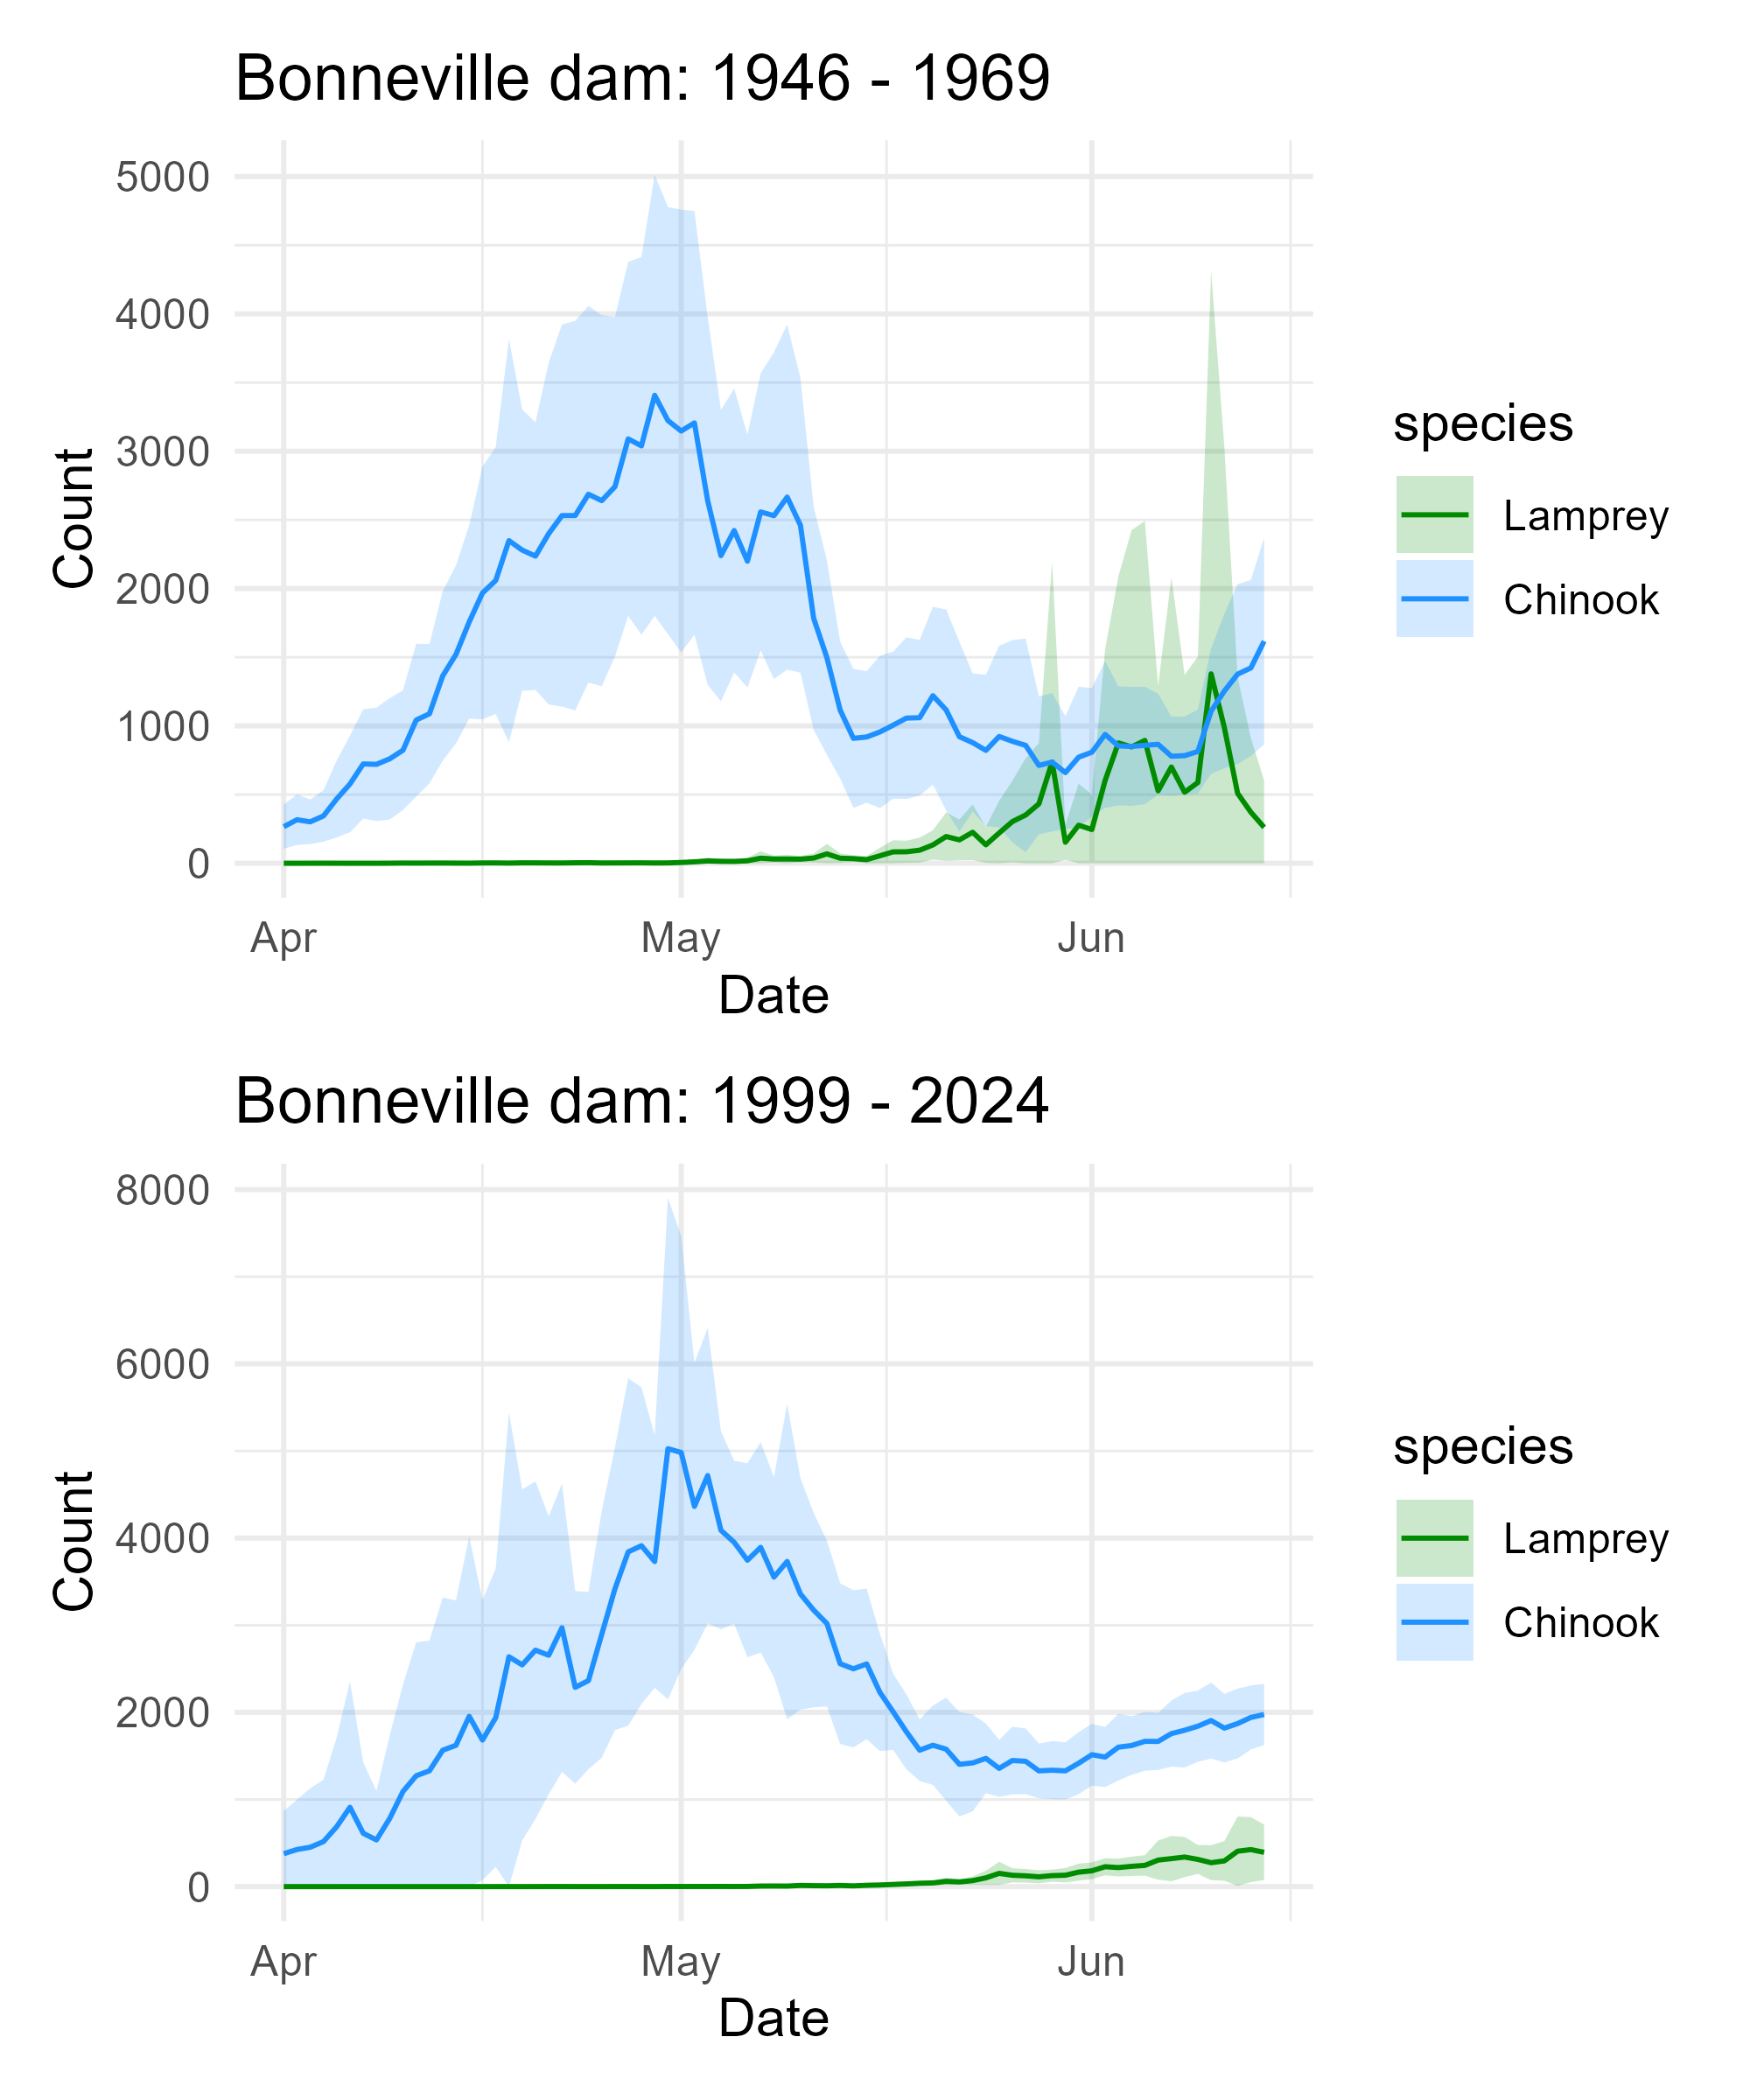
\includegraphics[width=0.8\linewidth]{../figures/supplemental/migration}

\textbf{Figure S1.} Count of Chinook salmon and Pacific lamprey passing
through Bonneville dam fish windows in April to mid-June from
\textbf{A.} 1946 - 1969 and \textbf{B.} 1999 - 2024. Pacific lamprey
counts were not recorded from 1970 - 1998. Solid line indicates the mean
count across years, and shaded area indicates \(\pm\) 0.5 standard
deviation from the mean.

\newpage

\pandocbounded{\includegraphics[keepaspectratio]{supporting_information_files/figure-latex/unnamed-chunk-33-1.pdf}}

\textbf{Figure S2.} Trace plots of posterior samples of MSFR parameters.
Colors refer to separate chains.

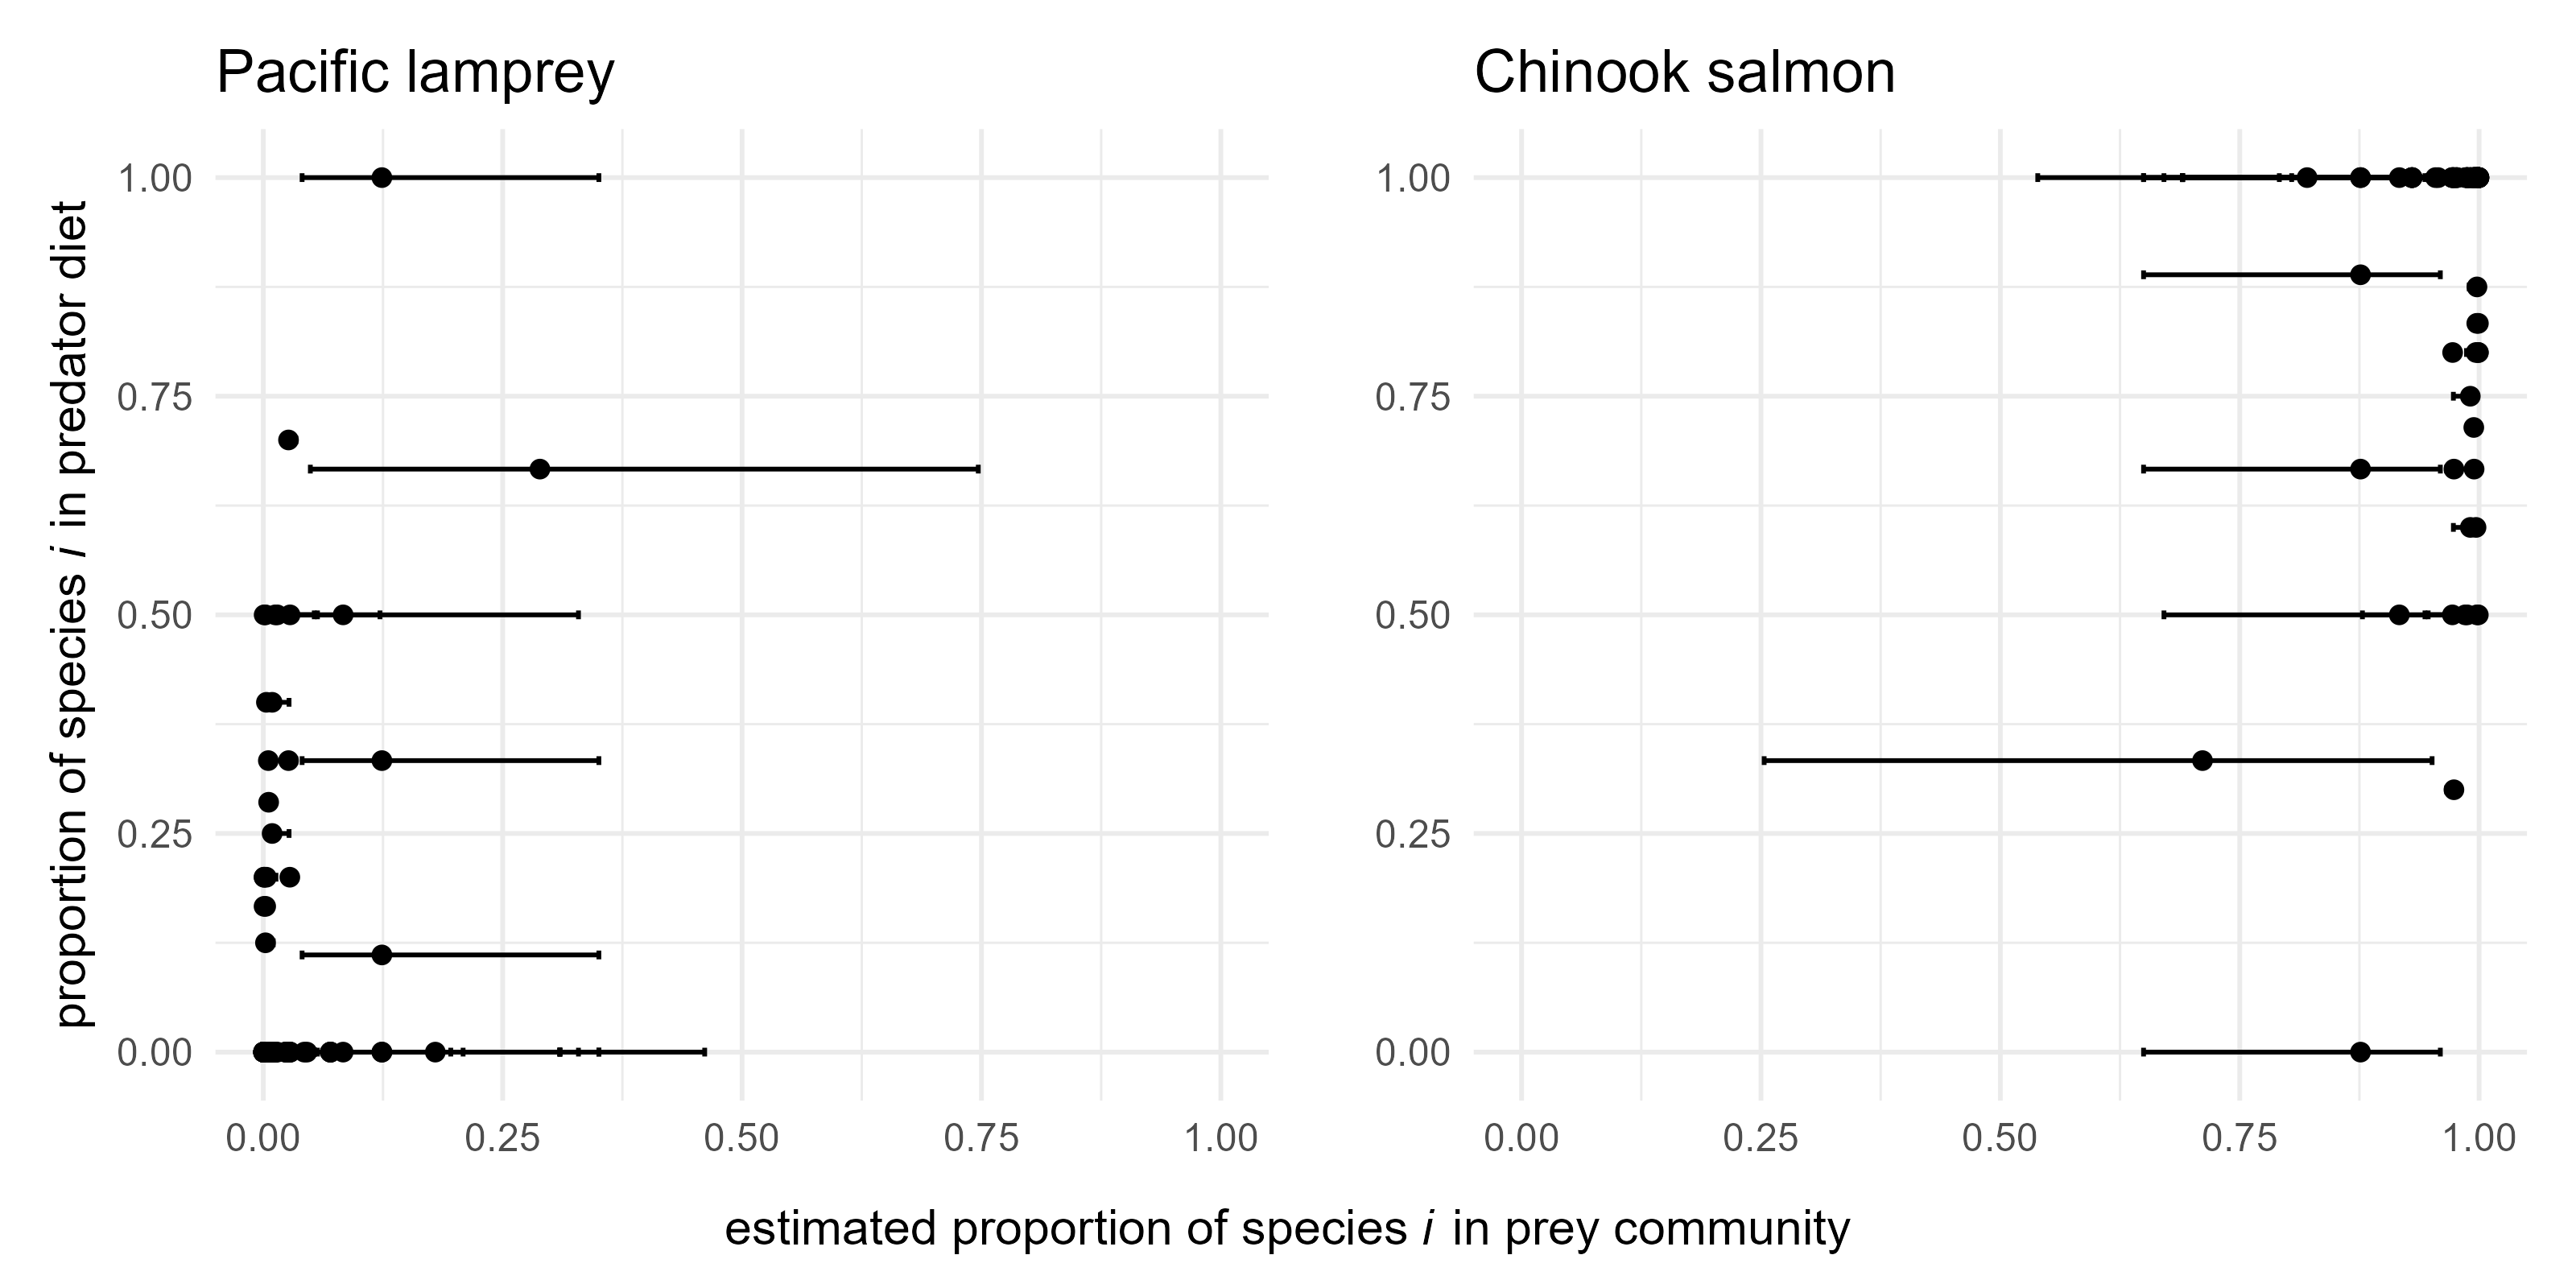
\includegraphics[width=0.8\linewidth]{../figures/supplemental/MSFR_nofit_error}

\textbf{Figure S3.} Relationship between the proportion of each fish
species in the predator's diet and estimated proportion of each fish
species in the prey community. Error bars indicate the 95\% credible
interval for the abundance of available lamprey and salmon, \(L^A_t\)
and \(S^A_t\), respectively.

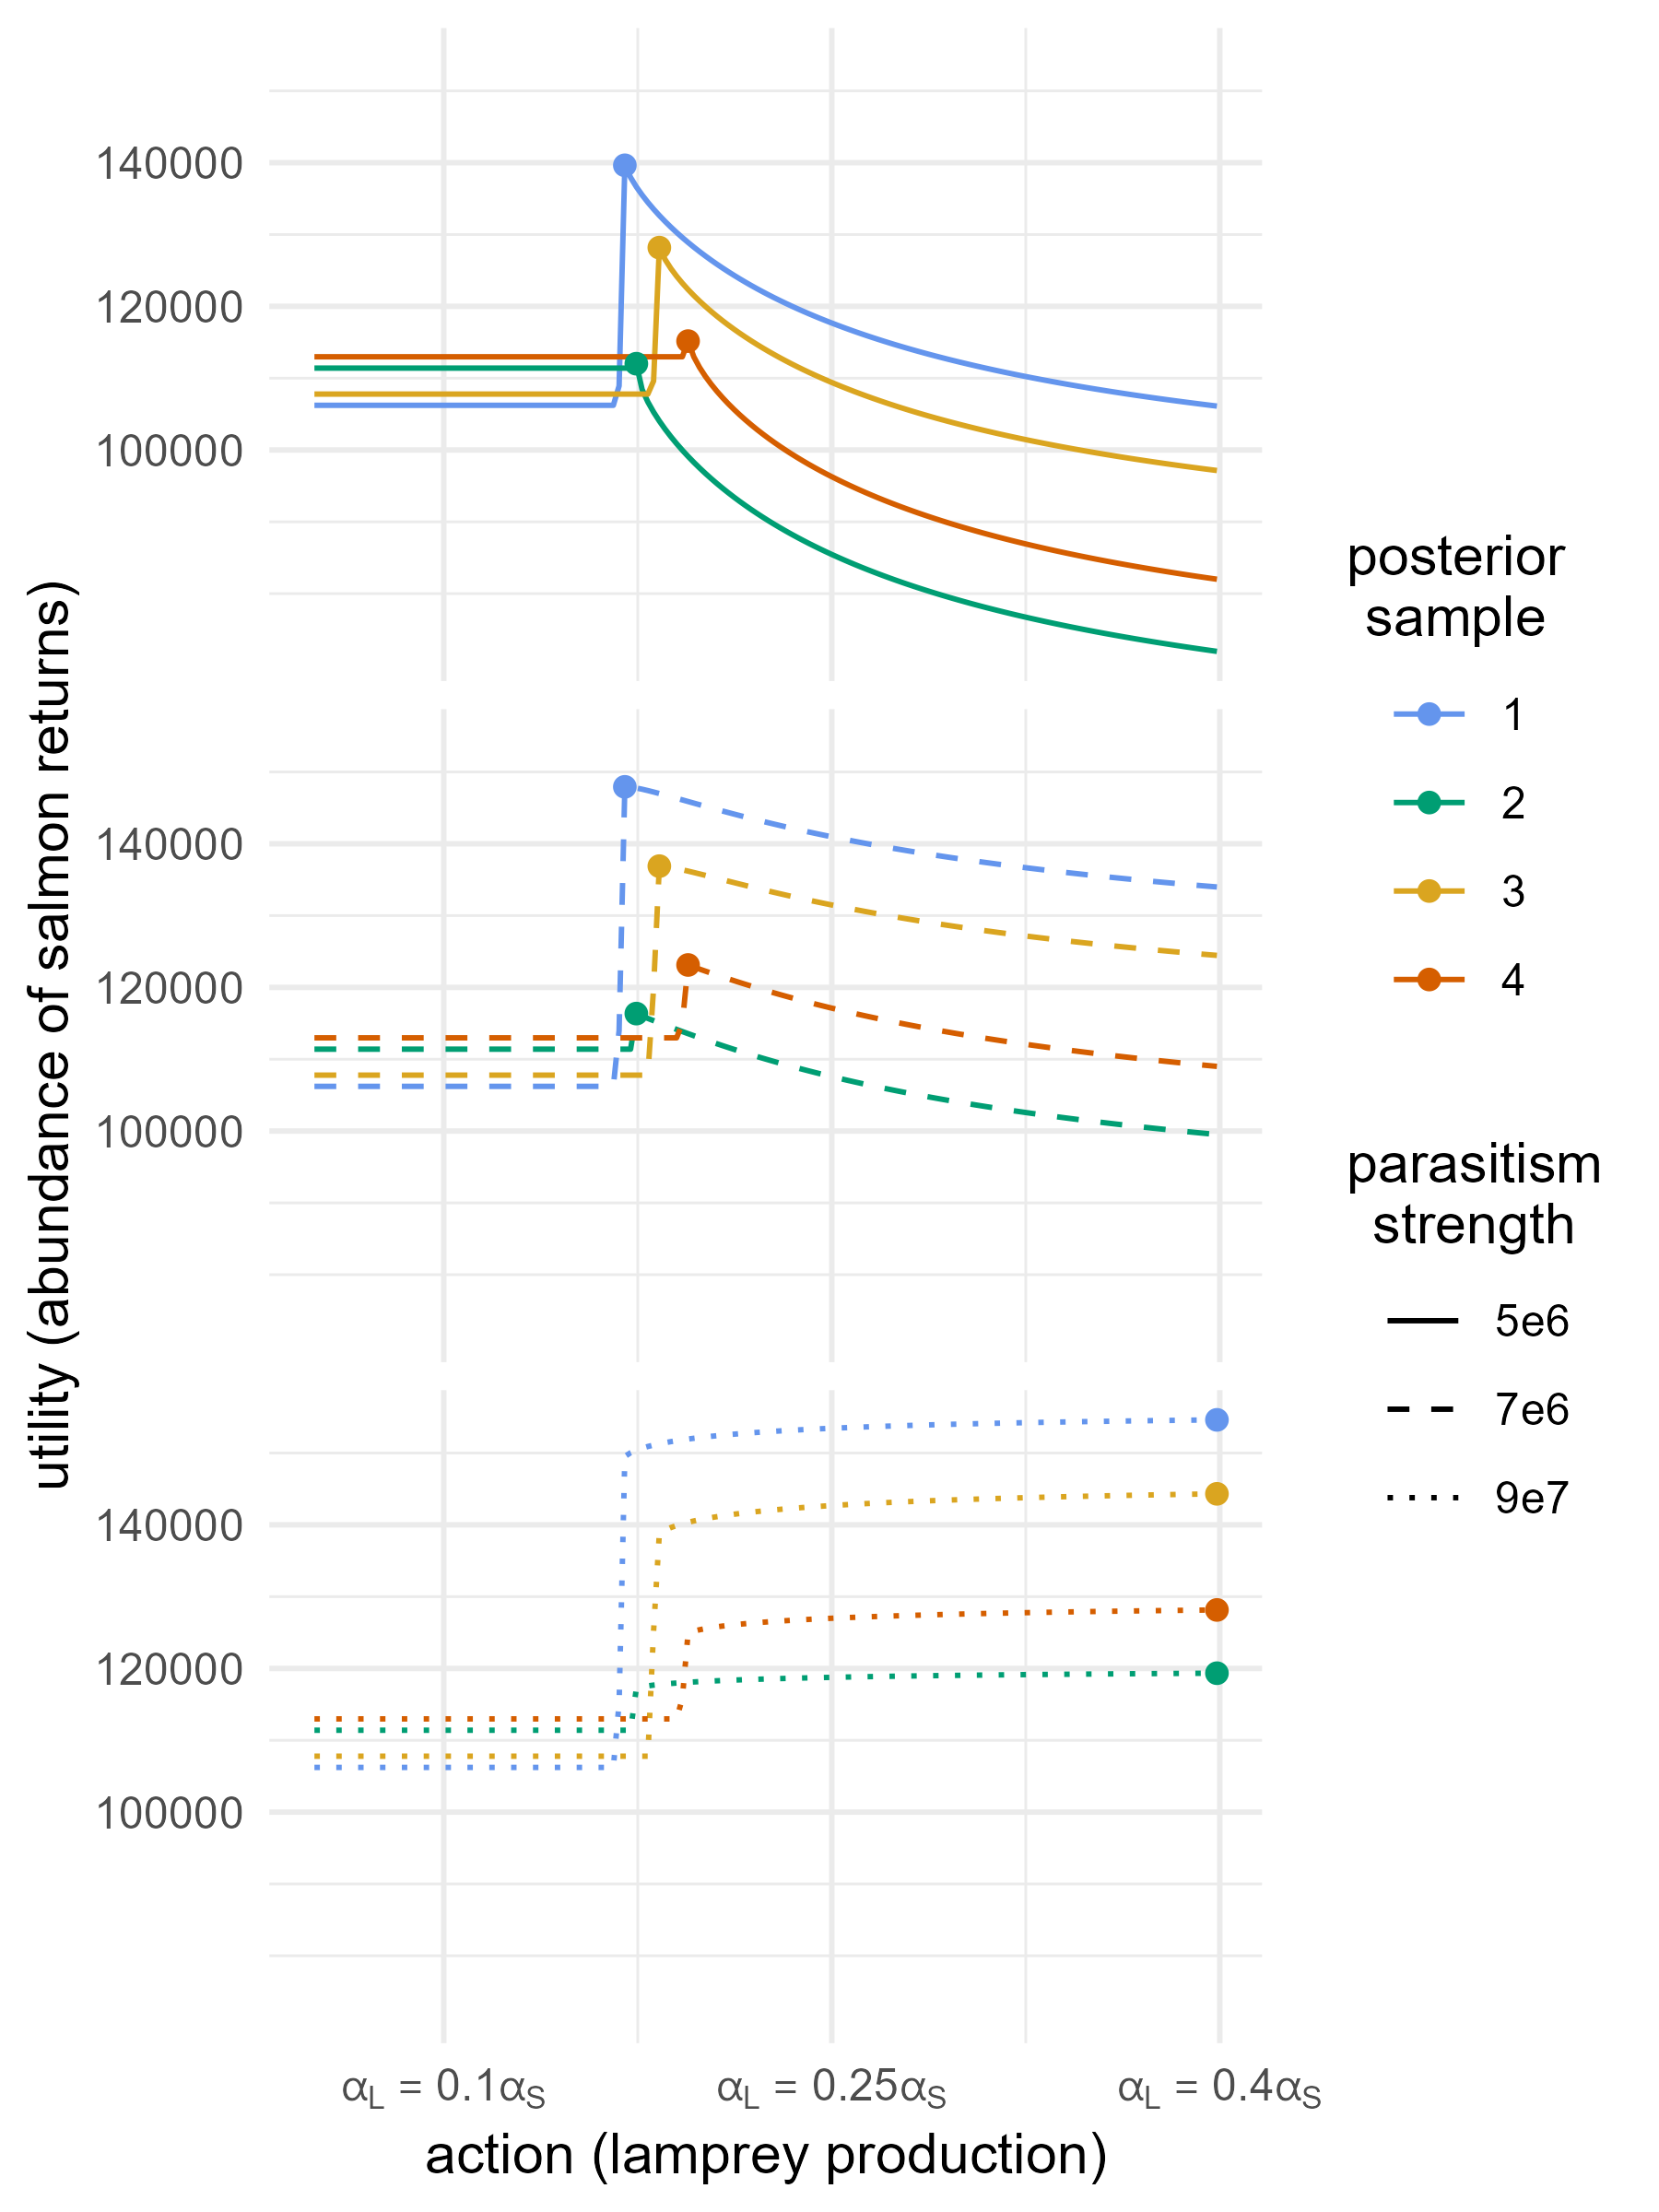
\includegraphics[width=0.8\linewidth]{../figures/supplemental/timeseries_equilibria}

\textbf{Figure S4.} Decision utility as a function of a decision maker's
action, or the lamprey production, \(\alpha_L\), relative to Chinook
salmon production, \(\alpha_S\). Colors correspond to functional
response uncertainty, and line types correspond to parasitism
uncertainty. The point indicates the action that maximizes utility,
\(a*\).

\newpage

\includegraphics[width=0.8\linewidth]{../figures/supplemental/supplemental_full_posterior-01}

\textbf{Figure S5.} Relationship between functional response uncertainty
and decision utility. \textbf{A.} Full posterior describing the
relationship between a species' proportion in the prey community and
proportion in the predator's diet for Pacific lamprey and Chinook
salmon. Each line corresponds to the MSFR prediction for each posterior
sample, and color corresponds to the value of each prediction when the
species' proportion in the prey community equals 0.5. Dashed black line
indicates the 1:1 line \textbf{B.} Decision utility calculated with each
sample from the full MSFR posterior in panel A. The expected utility is
calculated for each action, \(a \in A\) (lamprey production parameter,
\(\alpha_L\), relative to Chinook salmon production parameter,
\(\alpha_S\)). The asterisk indicates that the utility is calculated as
an expectation over parasitism uncertainty (i.e., \(E_P[U(a,f,p)]\)).
Points indicate the action that maximizes utility over parasitism
uncertainty (i.e., \(\text{max}_aE_P[U(a,f,p)]\)). Colors indicate the
corresponding posterior sample from panel A. The black line indicates
the utility calculated as an expectation over both parasitism and
functional response uncertainty (i.e., \(E_{F,P}[U(a,f,p)]\)). The black
point indicates the action that maximizes utility over all uncertainty,
or the bet-hedging strategy (i.e., \(\text{max}_aE_{F,P}[U(a,f,p)]\)).

\newpage

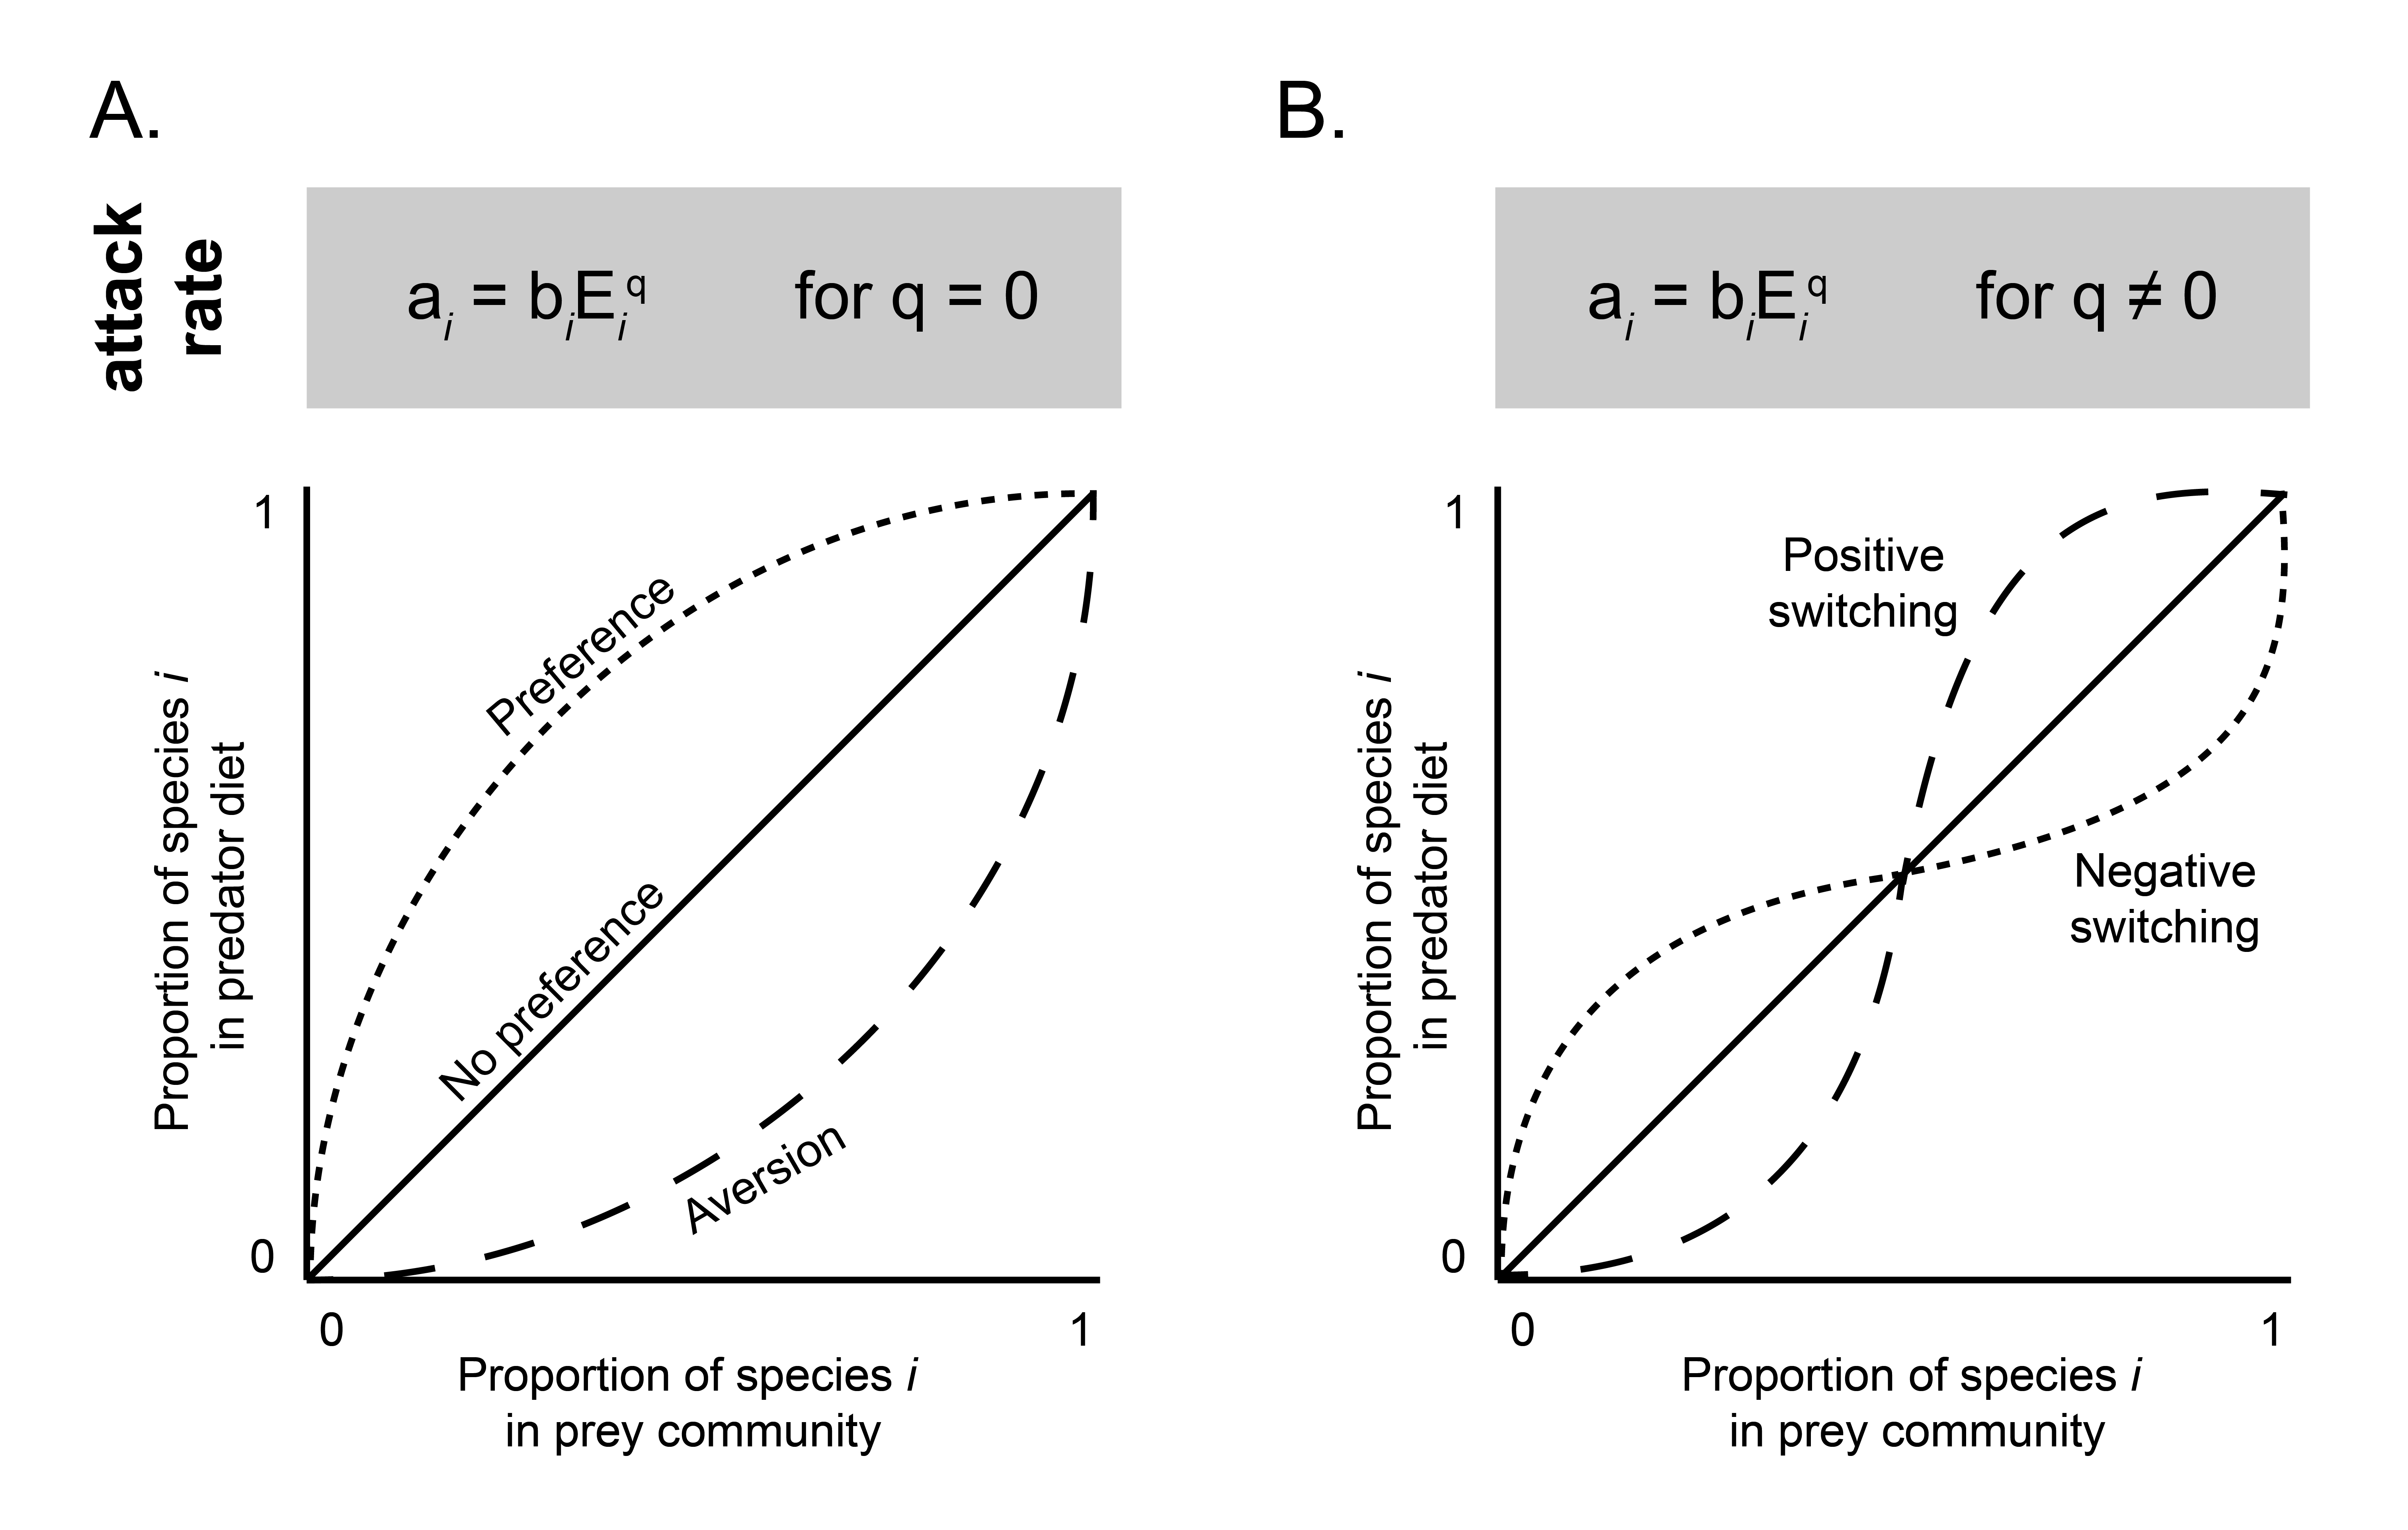
\includegraphics[width=0.8\linewidth]{../figures/supplemental/MSFR_conceptual_figure-01}

\textbf{Figure S6.} Conceptual diagram of density-dependent
multi-species functional response (MSFR), relating the formulation of
the density-dependent attack rate (Equations 1-2) to system behavior.

\pandocbounded{\includegraphics[keepaspectratio]{supporting_information_files/figure-latex/unnamed-chunk-38-1.pdf}}

\textbf{Figure S7.} Histogram of the proportion of lamprey observed by
visual day-time counts (\(C_V / C_T\)) is used to inform beta
distribution parameters, \(\alpha_D\) and \(\beta_D\) (Equation 13).

\includegraphics[width=0.8\linewidth]{supporting_information_files/figure-latex/unnamed-chunk-40-1}

\textbf{Figure S8:} Total count of Spring Chinook salmon passing through
Bonneville dam. Dashed red line indicates time series mean.

\newpage

\includegraphics[width=0.8\linewidth]{supporting_information_files/figure-latex/unnamed-chunk-42-1}

\textbf{Figure S9:} Relationship between salmon smolt abundance,
\(J_S\), and lamprey ocean survival (\(E_L / J_L\)), given parameter
value selected for \(D_L\), the coefficient scaling the rate at which
lamprey survival increases as a function of salmon density.

\newpage

\pandocbounded{\includegraphics[keepaspectratio]{supporting_information_files/figure-latex/unnamed-chunk-43-1.pdf}}

\textbf{Figure S10:} Data sources used to inform ocean mortality,
\(\phi\). \textbf{A.} Mean smolt-to-adult ratio (Bonneville dam juvenile
to Bonneville dam adult) calculated with PIT-Tagged Snake River
Spring/Summer Chinook ecologically significant unit (ESU), retrieved
from the DART data base. Red dashed line indicates time series mean
(\(R^\text{SAR}\) = 0.017). \textbf{B.} Annual estimated number of
spring run Chinook salmon lost to sources other than harvest between the
Columbia River Estuary and Bonneville Dam (retrieved from Table 5 in
(Wargo Rub et al. 2019)) Red dashed line indicates time series mean
(\(s^e\) = 0.26). The value we use for mortality in the ocean, \(\phi\)
is therefore: \(\phi = R^\text{SAR} / s^e = 0.06\).

\newpage

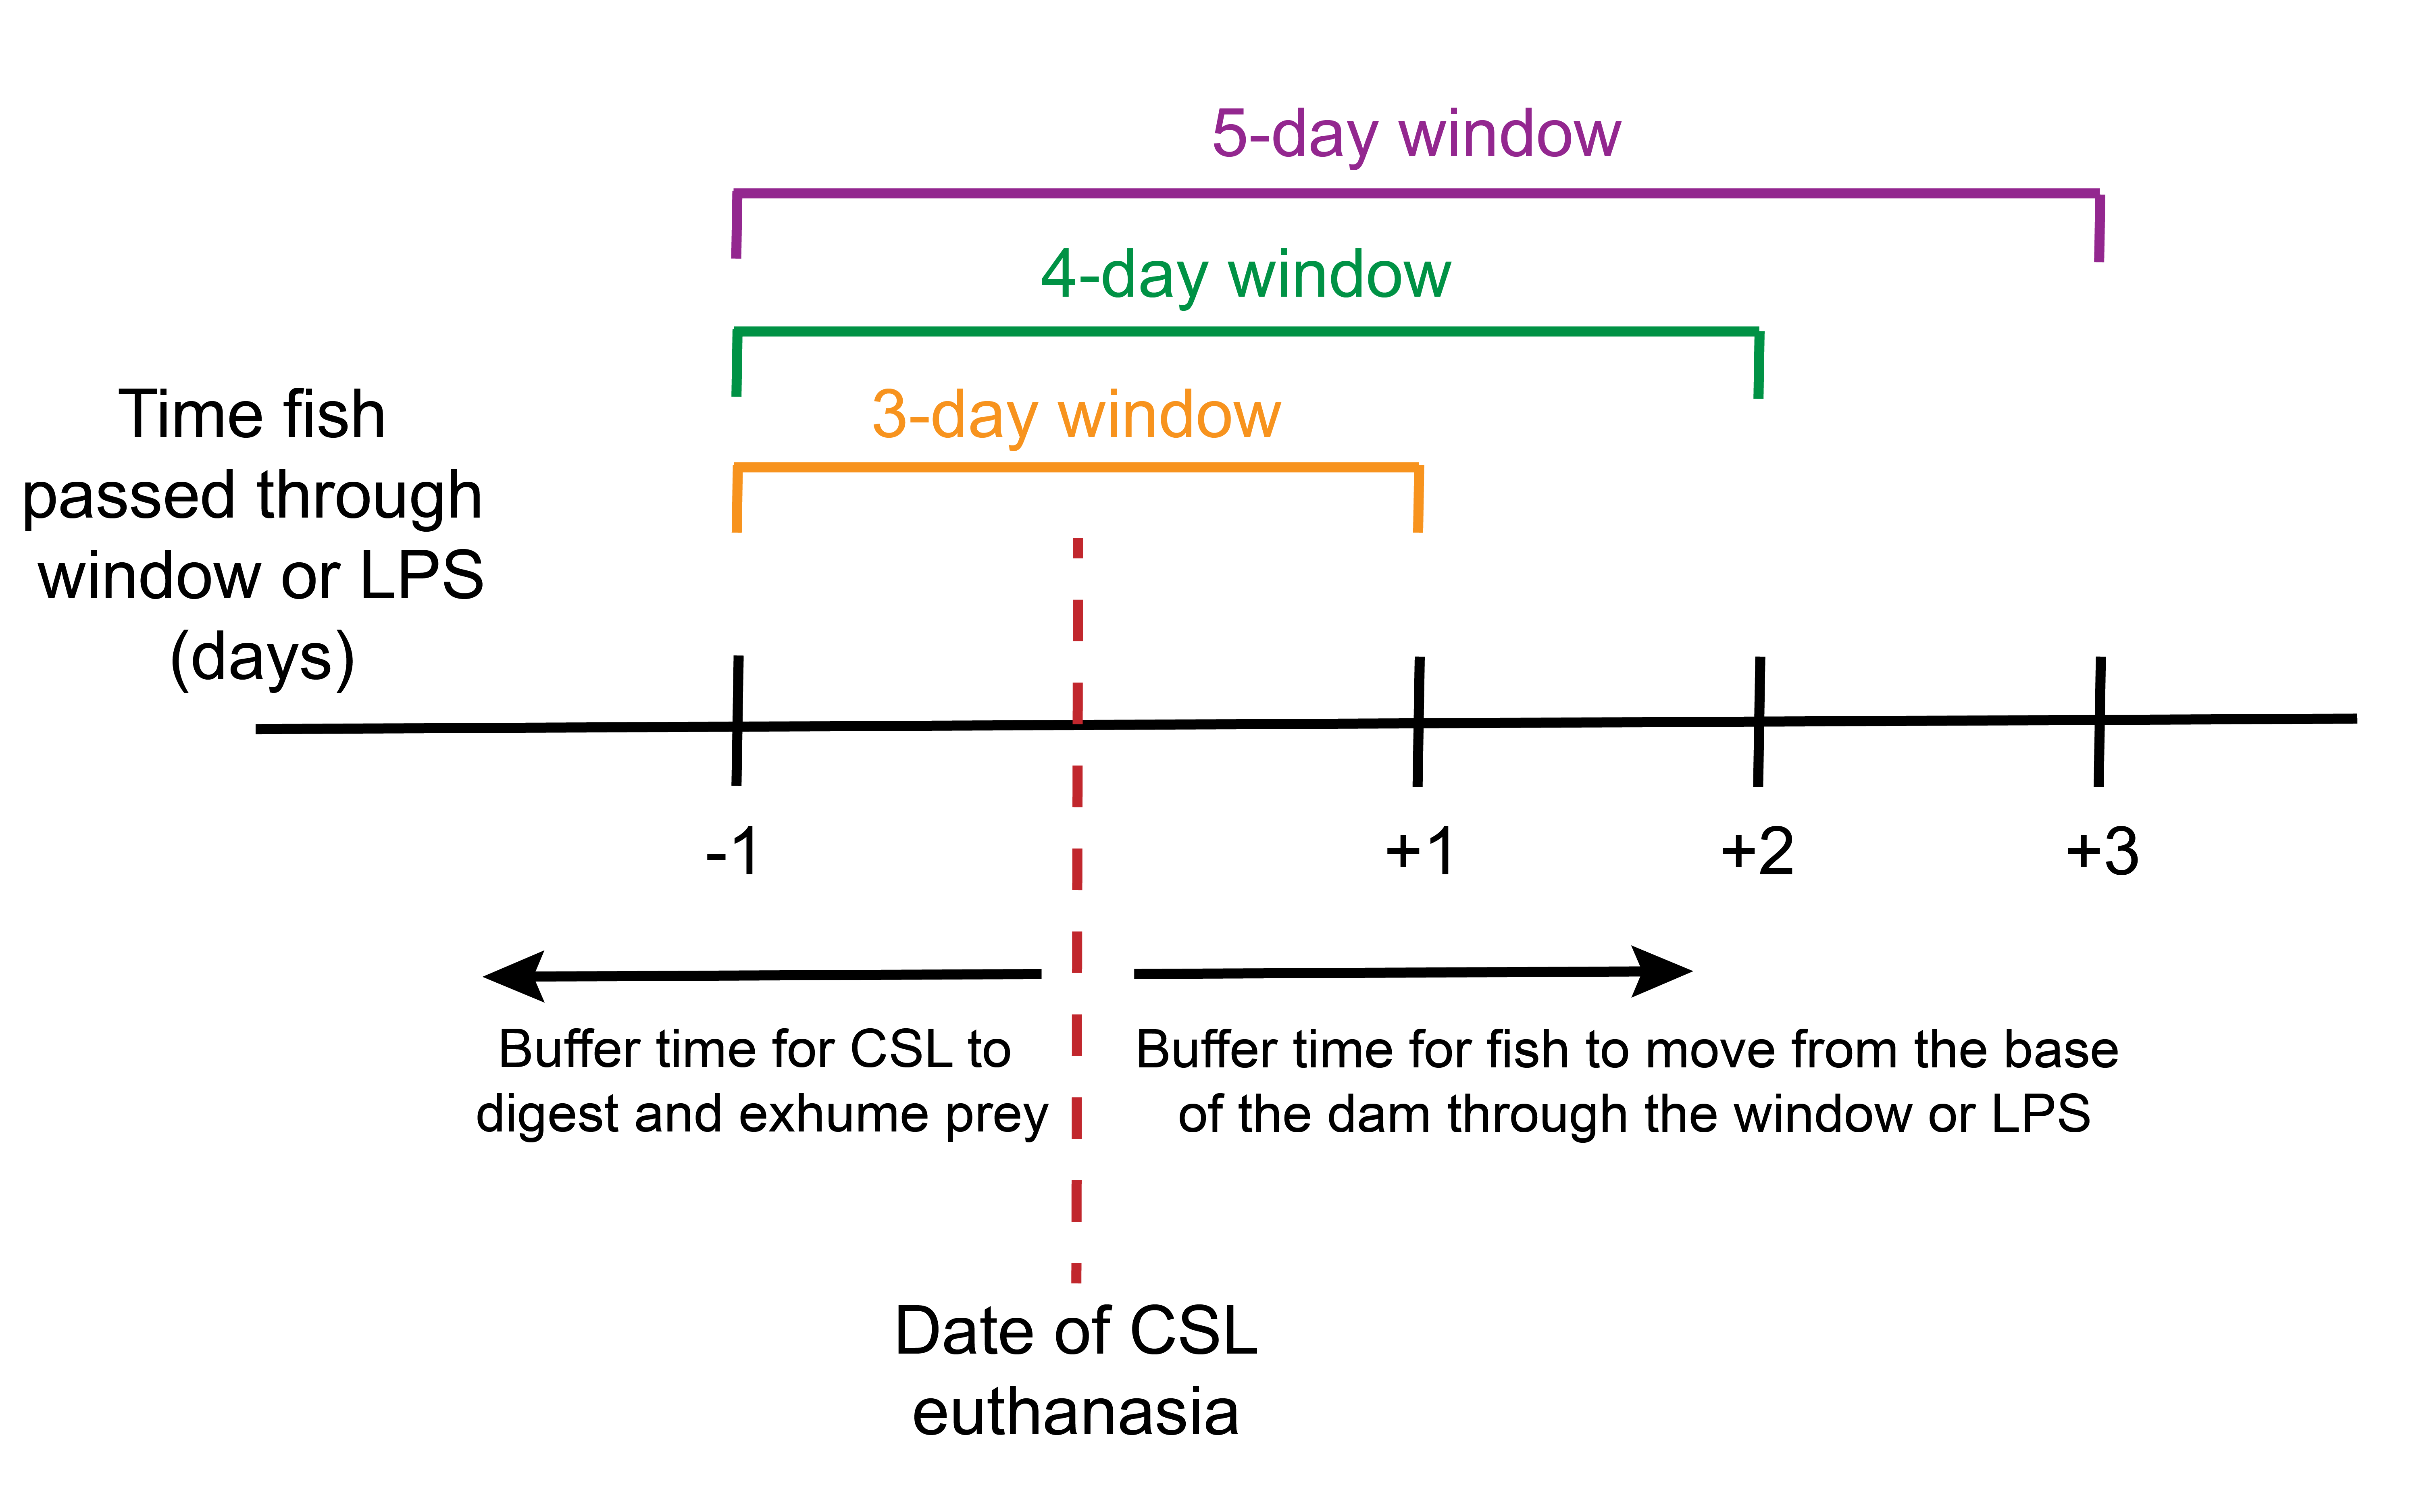
\includegraphics[width=0.8\linewidth]{../figures/supplemental/time_window-01}

\textbf{Figure S11.} Conceptual diagram of time window used to find the
sum of fish passing through the dam for each CSL euthanasia time point.
The axis is the time fish passed through the visual fish windows or
lamprey passage structures (LPS), measured in days.

\newpage

\pandocbounded{\includegraphics[keepaspectratio]{supporting_information_files/figure-latex/unnamed-chunk-47-1.pdf}}

\pandocbounded{\includegraphics[keepaspectratio]{supporting_information_files/figure-latex/unnamed-chunk-48-1.pdf}}

\pandocbounded{\includegraphics[keepaspectratio]{supporting_information_files/figure-latex/unnamed-chunk-49-1.pdf}}

\textbf{Figure S12.} Multi-species functional response (MSFR) model fits
of sensitivity analysis with 1000 randomly selected posterior samples
using the posterior from the \textbf{A.} 3-day time window (main
analysis results), \textbf{B.} 4-day time window, and \textbf{C.} 5-day
time window.

\section*{References}\label{references}
\addcontentsline{toc}{section}{References}

\phantomsection\label{refs}
\begin{CSLReferences}{1}{0}
\bibitem[\citeproctext]{ref-beamish1980adult}
Beamish, Richard J. 1980. {``{Adult biology of the river lamprey
(\emph{Lampetra ayresi}) and the Pacific lamprey (\emph{Lampetra
tridentate}) from the Pacific coast of Canada}.''} \emph{Canadian
Journal of Fisheries and Aquatic Sciences} 37 (11): 1906--23.

\bibitem[\citeproctext]{ref-brooks1998general}
Brooks, Stephen P, and Andrew Gelman. 1998. {``General Methods for
Monitoring Convergence of Iterative Simulations.''} \emph{Journal of
Computational and Graphical Statistics} 7 (4): 434--55.

\bibitem[\citeproctext]{ref-cates2020lamprey}
Cates, R. I. E., N. A. McClain, and K. M. Gibbons. 2020. {``{Use of
Adult Pacific Lamprey Passage Structures at Bonneville and John Day
Dams, 2019 Annual Report}.''} Technical Report. Cascade Locks, OR: U.S.
Army Corps of Engineers, Portland District, Fisheries Field Unit.

\bibitem[\citeproctext]{ref-clark2021pinniped}
Clark, Casey, Mike Brown, Doug Hatch, and Joe Dupont. 2021. {``Final
Field Report: 2017--2021 Pinniped Research and Management Activities at
Bonneville Dam.''} Final Field Report. Oregon Department of Fish;
Wildlife; Washington Department of Fish; Wildlife; Columbia River
Inter-Tribal Fish Commission; Idaho Department of Fish; Game.

\bibitem[\citeproctext]{ref-clark2023columbia}
Clark, Casey, John Edwards, Mike Brown, Shay Valentine, Bryan Wright,
Doug Hatch, John Whiteaker, and John Powell. 2023. {``Annual Report:
2023 Columbia River Basin Research and Management Activities.''} Annual
Report. Oregon Department of Fish; Wildlife; Washington Department of
Fish; Wildlife; Columbia River Inter-Tribal Fish Commission; Idaho
Department of Fish; Game.

\bibitem[\citeproctext]{ref-de2017programming}
de Valpine, Perry, Daniel Turek, Christopher J Paciorek, Clifford
Anderson-Bergman, Duncan Temple Lang, and Rastislav Bodik. 2017.
{``Programming with Models: Writing Statistical Algorithms for General
Model Structures with NIMBLE.''} \emph{Journal of Computational and
Graphical Statistics} 26 (2): 403--13.

\bibitem[\citeproctext]{ref-edwards2022columbia}
Edwards, John, Bryan Wright, Casey Clark, Mike Brown, Shay Valentine,
Doug Hatch, and John Powell. 2022. {``Annual Report: 2022 Columbia River
Basin Research and Management Activities.''} Annual Report. Oregon
Department of Fish; Wildlife; Washington Department of Fish; Wildlife;
Columbia River Inter-Tribal Fish Commission; Idaho Department of Fish;
Game.

\bibitem[\citeproctext]{ref-hatch2018sealion}
Hatch, Douglas R., Robert Lessard, and John M. Whiteaker. 2018. {``Sea
Lion Monitoring and Non-Lethal Hazing, 1/1/2018 -- 12/31/2018 Annual
Report.''} Project 2009-004-00.

\bibitem[\citeproctext]{ref-lance2001pinniped}
Lance, M. M. et al. 2001. {``Pinniped Food Habits and Prey
Identification Techniques Protocol.''} AFSC Processed Report 2001-04.
7600 Sand Point Way NE, Seattle, WA 98115: Alaska Fisheries Science
Center, NMFS, NOAA.

\bibitem[\citeproctext]{ref-murauskas2013relationships}
Murauskas, Joshua G, Alexei M Orlov, and Kevin A Siwicke. 2013.
{``Relationships Between the Abundance of {P}acific Lamprey in the
{C}olumbia River and Their Common Hosts in the Marine Environment.''}
\emph{Transactions of the American Fisheries Society} 142 (1): 143--55.

\bibitem[\citeproctext]{ref-Rcore}
R Core Team. 2025. \emph{R: A Language and Environment for Statistical
Computing}. Vienna, Austria: R Foundation for Statistical Computing.
\url{https://www.R-project.org/}.

\bibitem[\citeproctext]{ref-ransijn2021integrating}
Ransijn, Janneke M, Philip S Hammond, Mardik F Leopold, Signe Sveegaard,
and Sophie C Smout. 2021. {``Integrating Disparate Datasets to Model the
Functional Response of a Marine Predator: A Case Study of Harbour
Porpoises in the Southern North Sea.''} \emph{Ecology and Evolution} 11
(23): 17458--70.

\bibitem[\citeproctext]{ref-tidwell2023pinniped}
Tidwell, K. S., M. W. Braun, and B. K. van der Leeuw. 2023.
{``{Evaluation of Pinniped Predation on Adult Salmonids and Other Fish
in the Bonneville Dam Tailrace, 2022}.''} Technical Report. Cascade
Locks, OR: U.S. Army Corps of Engineers, Portland District, Fisheries
Field Unit.

\bibitem[\citeproctext]{ref-wargo2019changes}
Wargo Rub, A Michelle, Nicholas A Som, Mark J Henderson, Benjamin P
Sandford, Donald M Van Doornik, David J Teel, Matthew J Tennis, Olaf P
Langness, Bjorn K van der Leeuw, and David D Huff. 2019. {``{Changes in
adult Chinook salmon (\emph{Oncorhynchus tshawytscha}) survival within
the lower Columbia River amid increasing pinniped abundance}.''}
\emph{Canadian Journal of Fisheries and Aquatic Sciences} 76 (10):
1862--73.

\bibitem[\citeproctext]{ref-weitkamp2015seasonal}
Weitkamp, Laurie A, Susan A Hinton, and Paul J Bentley. 2015.
{``Seasonal Abundance, Size, and Host Selection of {W}estern {R}iver
(\emph{Lampetra Ayresii}) and {P}acific (\emph{Entosphenus Tridentatus})
Lampreys in the {C}olumbia {R}iver Estuary.''} \emph{Fishery Bulletin}
113 (2): 213--26.

\end{CSLReferences}

\end{document}
